\documentclass[conference,onecolumn]{IEEEtran}
\usepackage{setspace}
\onehalfspacing
\usepackage{acronym}
\usepackage[backend=bibtex]{biblatex}
\usepackage{graphicx}
\usepackage{csquotes}
\usepackage{hyperref}
\usepackage[margin=3cm]{geometry}
\usepackage[english]{babel}
\usepackage{float} % Added to support [H] float option
\graphicspath{ {./figures/} }
\addbibresource{../master-thesis.bib}
\newcommand{\code}[1]{\texttt{#1}}
\pagestyle{plain}
\begin{document}

  \begin{titlepage}


\raggedleft

\vspace*{-4cm}

\hspace*{8cm}

\includegraphics{uni-logo.png}

\centering
\Large
\department  
\vspace{0.5cm}\\

\normalsize
Software engineering group \\
June 29, 2025

\vspace{1.5cm}
\LARGE
Creating web-based diagram editors for specifying and executing model transformations

\vspace{1cm}
\Large
Master thesis

\vspace*{\fill}

\Large
from

\vspace{0.5cm}
\LARGE
Florian Weidner \vspace{1cm}

\vspace{1cm}

\vspace*{\fill}

\end{titlepage}

  \newpage

  \begin{abstract}
  lipsum bla bla bla
  \end{abstract}

  % \begin{IEEEkeywords}
  %   \acp{vit}
  % \end{IEEEkeywords}

  \IEEEpeerreviewmaketitle

    \newpage

 \tableofcontents
  \newpage

  \chapter{Introduction}
\label{sec:introduction}

\section{Background and Motivation}
\label{subsec:motivation}

In software engineering, often \ac{mde} is used to increase development productivity and quality. \cite{transformations-modeldriven} Concepts are modeled closer to the domain, so that they describe important aspects of a solution with human-friendly abstractions. The models can also be used to generate application fragments, that can be directly used as a template source code. In the process of \ac{mde}, many activities need to transform source models into different target models, while following a set of transformation rules. This model transformation process is based on algebraic graph transformations. A metamodel is used to model the structure and rules of the concept. The resulting transformation language can provide automatic model creation, development, and maintenance activities. \cite{transformations-modeldriven} One framework to use \ac{mde} is \ac{emf} by the Eclipse Foundation. It provides a basis for application development, using modeling and code generation facilities. Many frameworks build upon \ac{emf}, providing various \ac{mde} tools like code generators, graphical diagramming, model transformation, or model validation. \cite{emf} One model transformation framework is Henshin. \cite{henshin-repo} It tries to provide model transformation capabilities with a high level of usability. \cite{henshin-usability} For metamodels it uses \ac{emf} Ecore files. The framework allows to create and apply model transformations on XMI instance files with a defined transformation language. It provides a graphical and textual syntax to create these transformation rules. \cite{henshin-repo} Henshin can be used as a Eclipse plugin. For new users, Eclipse \acs{ide} needs to be installed and the heavy editor makes the use of Henshin unintuitive without prior experience.
Therefore, the goal exists to create a graphical option to use the Henshin model transformations without the overhead of the heavy \acs{ide}, that has to be installed. A web-based graphical editor would make the use of Henshin even more accessible and intuitive.

\ac{glsp} is a open-source framework by the Eclipse Foundation, which can be used to build a web-based Henshin graph editor. The framework is used to develop custom diagram editors for distributed web-applications. \cite{glsp-repo} It can provide graph editors for the Eclipse Desktop IDE, Eclipse Theia, \ac{vscode} and a stanalone version usable in any website. It brings the support of \ac{emf} models as a data source and the functionality of the Henshin SDK can be called from the Java server of \ac{glsp}. \cite{glsp-doc} With these functionalities, \ac{glsp} fits to create an easy accessible, intuitive application to create and apply Henshin model transformations called \textit{Henshin Web}.

\section{Problem Statement}
\label{subsec:problem-statement}

Despite the powerful capabilities of Henshin for model transformations, its current usage presents barriers to adoption and accessibility. The framework is exclusively available as an Eclipse \ac{ide} plugin, which requires users to install and configure the complete Eclipse environment before they can begin working with model transformations. This dependency limits the framework's reach and usability.

First, the requirement for Eclipse installation presents a substantial entry barrier, particularly for newcomers to \ac{mde} who wish to explore model transformation concepts without committing to a full development environment setup. For example, students or researchers who want to quickly experiment with Henshin transformation rules face unnecessary complexity in simply accessing the tool. The installation process, environment configuration, and learning the Eclipse interface adds cognitive overhead that detracts from the Henshin functionality itself.

Second, the Eclipse \ac{ide} presents usability challenges. Eclipse is a heavyweight development environment with many features and a complex interface. It can feel overwhelming when the primary goal is to create and apply model transformations. Users must navigate through multiple perspectives, views, and menus to accomplish basic transformation tasks, leading to reduced productivity and increased frustration.
The standard editor for Ecore, Henshin rules and \ac{XMI} instance files is a tree view, which can get unintuitive for bigger models. In order to edit the transformation rules graphically, a diagram file needs to be initialized separately. To edit the Ecore metamodels, also the diagram has to be initialized specifically. For the \ac{xmi} instance files, an extension has to be installed. Especially the application of transformation rules is not supported graphically even with extensions, but only through a wizzard window.  

Furthermore, the current setup limits collaborative possibilities and portability. Sharing transformation examples across different clients or collaborating on transformation development is not possible with Eclipse. \ac{vcs} have to be used to share files and real-time collaboration or easy access from different devices is not supported.

These accessibility and usability challenges prevent Henshin from reaching its full potential as a model transformation solution, particularly for beginners who face significant initial challenges and among users who could benefit from quick, intuitive access to transformation capabilities without the overhead of a complete \ac{ide} setup.

\section{Research Questions}
\label{subsec:research-questions}

Based on the identified problems with the current Eclipse-based approach to Henshin model transformations, this thesis aims to address the following research questions that guide the development and evaluation of a web-based solution:

\textbf{RQ1: How can Henshin model transformation capabilities be effectively adapted for web-based environments?}
This question investigates the technical feasibility and architectural considerations for translating the desktop-based Henshin functionality into a web application. It examines how the core transformation engine, metamodel handling, and rule definition capabilities can be preserved while adapting to web technologies and browser constraints.


\textbf{RQ2: What are the essential functional requirements for a web-based Henshin editor that maintains usability while reducing complexity?}
This question focuses on identifying the minimum viable feature set that provides meaningful transformation capabilities in order to create an application that can completely handle typical use cases.


\textbf{RQ3: How does a web-based approach improve accessibility and user experience compared to the traditional Eclipse plugin?}
This question evaluates the effectiveness of the web-based solution in addressing the identified barriers to adoption. It examines metrics such as installation complexity, learning curve, collaboration capabilities, and overall user satisfaction when working with model transformations.


\textbf{RQ4: How do different deployment strategies affect the accessibility, usability, and adoption barriers for web-based model transformation tools?}
This question explores various deployment options for the web-based Henshin editor, such as standalone web applications, cloud-hosted services, or integration with existing platforms. It assesses how these strategies impact user access, ease of use, and the overall adoption of the tool among different stakeholder groups.


\textbf{RQ5: How can the web-based editor integrate with existing \ac{emf} and Henshin ecosystems?}
This question explores the compatibility and interoperability requirements for ensuring that the web-based solution can work with existing metamodels, transformation rules, and instance files created in the traditional Eclipse environment, while also providing value as an independent tool.

These research questions collectively address the goal of creating an accessible, intuitive, and functionally adequate web-based alternative to the current Eclipse-dependent Henshin workflow, while ensuring that the solution provides authentic value to the identified stakeholder groups.

\section{Scope and Limitations}
\label{subsec:scope-limitations}

This thesis focuses on developing a web-based solution for Henshin model transformations, with specific boundaries and constraints that define the research scope and acknowledge inherent limitations.

\textbf{Scope of the Research:}
The primary scope encompasses the design, implementation, and evaluation of a web-based editor that provides core Henshin transformation capabilities with the \ac{glsp} framework. The work includes adapting the essential features of the Henshin Eclipse plugin for web environments, focusing on transformation rule creation, metamodel handling, and instance file processing. The implementation targets the fundamental workflow of loading \ac{emf} Ecore metamodels, creating transformation rules through a graphical interface, and applying these transformations to \ac{xmi} instance files.

The research specifically addresses accessibility improvements to minimize the initial challenge for beginners, where users need quick access to model transformation capabilities without extensive setup requirements. The evaluation covers usability aspects, performance characteristics, and functional completeness compared to the traditional Eclipse-based approach. Integration with existing \ac{emf} and Henshin ecosystems is considered to ensure compatibility with established workflows and file formats.

\textbf{Limitations and Constraints:}
Several limitations constrain the scope of this research. The web-based implementation does not aim to replicate every advanced feature available in the mature Eclipse Henshin plugin. Complex transformation scenarios, advanced debugging capabilities are beyond the current scope. The focus remains on core functionality that serves the primary use cases identified in the requirements analysis.

The evaluation methodology is constrained by the availability of test scenarios and user groups within the academic environment. While the research aims to demonstrate improvements over the Eclipse approach, comprehensive studies or extensive industrial validation are outside the scope of this thesis work.

Additionally, the research does not extend to developing new transformation algorithms or enhancing the underlying Henshin transformation engine itself. The focus remains on providing better accessibility and usability for existing Henshin capabilities rather than advancing the theoretical foundations of model transformation techniques.

A system constraint is that the backend has to be Java-based, to be able to directly run the Henshin \acs{sdk}. 

These scope definitions and limitations ensure that the research remains focused and achievable within the constraints of a master's thesis while addressing the core problems identified in current Henshin usage patterns.

\section{Structure of the Thesis}
\label{subsec:structure-thesis}

This thesis is structured as follows, with each chapter building upon the previous ones to provide a comprehensive view of the development and evaluation of the Henshin Web application:

\textbf{Chapter \ref{sec:theoretical-background} - Theoretical Background} introduces the foundational technologies and concepts essential for understanding this work. It covers the Eclipse Foundation ecosystem, \ac{emf} as the modeling framework, Henshin for model transformations, and \ac{glsp} as the web-based graphical editing platform. This chapter establishes the technical context and terminology used throughout the thesis.

\textbf{Chapter \ref{sec:related-work} - Related Work} surveys the landscape of model transformation tools and web-based modeling solutions. It examines scientific literature on model transformation software, analyzes existing tools and their limitations, and compares various web-based modeling environments. This analysis positions Henshin Web within the broader context of available solutions and highlights the gap it aims to fill.

\textbf{Chapter \ref{sec:requirements} - Requirements} defines the functional and non-functional requirements for the Henshin Web editor. It identifies potential user groups, establishes the system scope and context, and details the specific capabilities the application must provide. This chapter serves as the foundation for design and implementation decisions made in subsequent chapters.

\textbf{Chapter \ref{sec:architecture} - Architecture} presents the overall system architecture of Henshin Web. It describes the structural design decisions, component interactions, and architectural patterns employed to meet the identified requirements. The chapter explains how the web-based architecture integrates with existing Henshin and \ac{emf} ecosystems while providing the desired accessibility improvements.

\textbf{Chapter \ref{sec:implementation} - Implementation} details the concrete implementation of core components within the Henshin Web application. It covers the technical realization of key features, integration challenges, and solutions developed to adapt Henshin capabilities for web environments. This chapter provides insight into the practical aspects of translating architectural designs into working software.

\textbf{Chapter \ref{sec:testing} - Testing and Evaluation} discusses the comprehensive testing strategy employed to validate the application's functionality and performance. It covers unit testing approaches, end-to-end testing methodologies, and evaluation criteria used to assess the system's effectiveness. The chapter also addresses testing limitations and their implications for the validation of research outcomes.

\textbf{Chapter \ref{sec:deployment} - Deployment} explores various deployment strategies and options for making Henshin Web accessible to users. It examines different hosting approaches, infrastructure requirements, and considerations for scalability and maintenance. This chapter addresses the practical aspects of delivering the solution to end users.

\textbf{Chapter \ref{chap:usage} - Usage} provides comprehensive user guidance for working with Henshin Web. It includes detailed user guides for creating and editing metamodels, transformation rules, and instance files, as well as administrative guidance for user management and system configuration. This chapter serves as practical documentation for both end users and system administrators.

\textbf{Chapter \ref{sec:discussion-conclusion} - Discussion and Conclusion} synthesizes the research findings, evaluates the success of the approach in addressing the identified problems, and reflects on the broader implications for web-based model transformation tools. It discusses limitations of the current implementation, potential future enhancements, and the contribution of this work to the field of model-driven engineering.

  \chapter{Background}
\label{sec:background}
  In this section, the theoretical background of the project and used technologies are described. First the Eclipse Foundation is introduced, as many used frameworks are developed under the Eclipse Foundation. Then, the Eclipse Modeling Framework is described, as it is the core of the used frameworks. After that, the model transformation language Henshin is introduced. Finally, the framework \ac{glsp} is described, that is used to create web-based diagram editors.

  \section{Eclipse Foundation}
  \label{subsec:eclipse-foundation}
  The Eclipse Foundation is a not-for-profit, member-supported corporation that provides an environment for individuals and organizations for collaborative and innovative software development. \cite{eclipse-review} The Eclipse Foundation grew out of the publication of the Eclipse \ac{ide} code from IBM in 2001. The Eclipse Foundation itself was founded in 2004. The new organization was founded to continue the development of Eclipse IDE as an open source platform. Over time, the organization initiated numerous projects in the Eclipse environment, all operating under the Eclipse Public License. \cite{heise-eclipse-foundation,eclipse-review} In the recent years, the key initiatives of the Eclipse Foundation are contributing to european digital sovereignty, enhancing security measures, innovating \ac{sdv}, organizing community events, and improving their most popular projects. Popular projects are for example the Jakarta EE, an ecosystem for cloud-native applications with java, Eclipse Temurin, providing open source Java Development Kits and the Eclipse IDE. \cite{eclipse-report} In total, the Eclipse Foundation hosts more than 400 open source projects, supported 14 european research projects in 2024, and has 117 organizations participating in commits. \cite{eclipse-report}

  The scope of this work remains within the Eclipse Foundation ecosystem. All frameworks used are projects from the Eclipse Foundation. The used frameworks are described in the sections \ref{subsec:emf}, \ref{subsec:henshin} and \ref{subsec:glsp}.

  The Eclipse \ac{ide} is not the main project, but it is still an important part of the Eclipse infrastructure. It is divided into four main components: Equinox, the Platform, the \ac{jdt} and the \ac{pde}. Together they provide everything to develop and extend Eclipse-based tools. Equinox and the Platform are the core of the Eclipse \ac{ide}. With expanding the core with the \ac{jdt} or other plugins, the \ac{ide} can be used to develop different programming languages, like Java, C/C++, or PHP. \cite{emf} Eclipse provides different packages to download, depending on the use case. One package is the Eclipse Modeling Tools package by the Eclipse Modeling Project. It provides tools and runtimes to build model-based applications. It can be used to graphically design domain models and test those models by creating and editing dynamic instances. Also, Java code can be generated from the models to get a scaffold that can be used to create applications on top. \cite{eclipse_modeling} The base of the Eclipse Modeling Tool is \ac{emf} (section \ref{subsec:emf}). Other modeling tools and projects that are built on top of the \ac{emf} core functionality provide capabilities for model transformation, database integration, or graphical editor generation. \cite{emf}

  \section{\acf{emf}}
    \label{subsec:emf}

    \begin{quote}
      \glqq\acf{emf} is a modeling framework and code generation facility for building tools and other applications based on a structured data model.\grqq{} \autocite{emf-repo}
    \end{quote}

    \acf{emf} is the core part of the Eclipse Modeling Project and unifies the representation of models in \acs{uml}, \acs{xml} and Java. You can define your model in one of these formats and use \ac{emf} to generate the other formats.
    
    \ac{emf} consists of three components. The \ac{emf} core part provides Ecore metamodels, runtime support for the models, and a basic \acs{api} for manipulating \ac{emf} objects generically. Ecore metamodels are used to describe the structure of a model. \cite{eclipse_emf} They can be serialized in \ac{xmi} 2.0, as Ecore \ac{xmi}, and have the file extension \textit{.ecore}. There are several Ecore classes to represent a model, here are the most important ones:

    \begin{itemize}
      \item \textbf{EClass}: A class in the model that is identified by a name, containing attributes and references to other classes. It can also refer to a number of other classes as its supertypes to support inheritance. \cite{emf}
      \item \textbf{EAttribute}: An attribute of a class, that are identified by a name and have a type. \cite{emf}
      \item \textbf{EDataType}: A simple data type like \code{EString}, \code{EBoolean} or \code{EJavaClass}. \cite{emf}
      \item \textbf{EReference}: A reference to another class, containing a link to an instance of that class. \cite{emf}
    \end{itemize}


    Together, \citeauthor{emf} called these classes the Ecore kernel. In Figure \ref{fig:emf-kernel} you can see the kernel classes and their relations. These classes are enough to define simple models. \textbf{EAttribute} and \textbf{EReference} have a lot of similarities. They both define the state of an instance of an \textbf{EClass} and have a name and a type. For that, Ecore provides a common interface for both, called \textbf{EStructuralFeature}. Ecore can also model behavioral features of classes as \textbf{EOperation} using \textbf{EParameter}. All classes have the common interface \textbf{EObject}, being the root of all modeled objects. Related classes are grouped into packages called \textbf{EPackage}. It is represented by the root element when the model is serialized. \cite{emf}

    \begin{figure}[h]
      \centering
      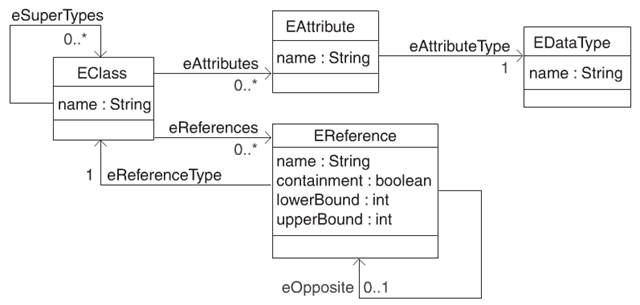
\includegraphics[width=0.7\textwidth]{emf-kernel}
      \caption{The Ecore kernel. Image obtained from \cite{emf}}
      \label{fig:emf-kernel}
    \end{figure}

    The second component of \ac{emf} is \ac{emf}.Edit. It provides generic reusable classes to build viewers and editors for \ac{emf} models. With these classes, \ac{emf} metamodels can be displayed in JFace viewers, that are part of the Eclipse \acs{ui}. \cite{eclipse_emf} The Eclipse \ac{ide} can display an Ecore model in a tree viewer. Eclipse accesses the data over the \code{ITreeContentProvider} interface to navigate the content and the \code{ILabelProvider} interface to provide the label text and icons for the displayed objects. The properties of objects are displayed in a Property Sheet over the \code{IPropertySourceProvider}, where the user can edit the model. \ac{emf}.Edit also provides undo and redo operations when creating or editing an instance model. For that, it uses a command framework with commands like an \code{AddCommand}, \code{SetCommand} or \code{CopyCommand}. \cite{emf}

    The third component is \ac{emf}.Codegen. It can generate Java code for a complete editor for \ac{emf} instance models of an Ecore metamodel. It provides different generation options. So, unlike \ac{emf}.Edit, that just provides generic classes for Ecore models, \ac{emf}.Codegen directly generates complete editors with a \acs{ui}. \cite{eclipse_emf} The generation can be done over a wizard in the Eclipse \ac{ide} or by using the command line interface. \cite{emf} The generation can be separated into three levels. The first level is to generate Java interfaces and implementations for the Ecore model classes and a factory- and package-implementation class. The second level generates specific \code{ItemProviders} to edit instance models based on the metamodel. The classes are structured like the \ac{emf}.Edit component for the Ecore models. The third level generates a structured editor with \acs{ui} that works like the Ecore editor in the Eclipse \ac{ide} and can be a starting point for customization. \cite{eclipse_emf} There are many frameworks that build on top of \ac{emf}, using these generation capabilities to create further modeling functionality. For model transformations the most popular frameworks that build upon \ac{emf} are Eclipse Acceleo, Eclipse VIATRA, Eclipse ATL, Eclipse QVT Operational, Eclipse QVT Declarative and Henshin \ref{subsec:henshin}.

  \section{Henshin}
  \label{subsec:henshin}

  One part of the Eclipse Modeling Project for model transformations is Henshin. It can be used as a plugin in the Eclipse \ac{ide} or as an \acs{sdk}. It provides a graphical and textual syntax to define model transformation rules and apply them to \ac{emf} XMI instance models. It can be used for endogenous transformations, where \ac{emf} model instances are directly transformed, and exogenous transformations, where new instances are generated from given instances using a trace model. It also brings efficient in-place execution of transformations using an interpreter with debugging support and a performance profiler. Henshin also provides conflict and dependency analysis, and state space analysis for verification. \cite{henshin-repo}

  Henshin builds on top of \ac{emf}. It uses an Ecore metamodel to define the structure of the transformation rules, resulting in a serialized \ac{xmi} file with the file extension \textit{.hensin}, that can therefore be edited in the Eclipse tree editor. \cite{henshin-repo} The metamodel of the transformation rules uses another Ecore metamodel that models the model structure of the domain, to type the nodes, egdes, and attributes of the rules. \cite{henshin} In Figure \ref{fig:henshin-rule-model} you can see the Henshin transformation rule metamodel. A rule consists of a \ac{rhs} graph, a \ac{lhs} graph and attribute conditions. Additionally, mappings between the \ac{lhs} and \ac{rhs} graph are defined between nodes. The mapping of the edges is done implicitly by the mapping of the source and target nodes. \cite{henshin} Henshin uses units to control the order of rule applications. With units, control structures can be defined. Also, parameters can be passed from the previous executed rule to the next one to have a controlled object flow. Henshin's tansformation language is based on algebraic graph transformations, complying with the syntactical and semantic structure of rules and transformation units. This ensures a language usable for formal verification or validation. \cite{henshin}

  In the Eclipse \ac{ide}, rules can also be edited in a graphical editor. The rules are displayed as a single graph, calculated from the \ac{lhs} and \ac{rhs} graphs. The nodes and edges are annotated with \textit{\textless{}\textless{}preserve\textgreater\textgreater}, \textit{\textless{}\textless{}create\textgreater\textgreater}, \textit{\textless{}\textless{}delete\textgreater\textgreater}, \textit{\textless{}\textless{}forbid\textgreater\textgreater} or \textit{\textless{}\textless{}require\textgreater\textgreater} to indicate what happens to the nodes and edges when applying the rule. These annotations can be directly edited in the graphical editor and the the \ac{lhs} and \ac{rhs} graphs are then adapted to the change. Also, multiple \acp{nac}, \acp{pac} and parameters can be specified directly. \cite{henshin-repo} When a set of transformation rules are specified, they can be applied to an \ac{emf} \ac{xmi} instance model, by using a wizard in the Eclipse \ac{ide}. There, the source model, the rule, and its parameters can be selected. The result of the transformation can be seen in a new \ac{xmi} instance file. \cite{henshin-repo} Next to the graphical editor, Henshin also provides a textual syntax to define transformation rules and units. In a \textit{.henshin\_rule} file with the keyword \textbf{rule} a name and parameters, a new rule can be described. If you want to define a node, you can use the keyword \textbf{node} with a action keyword like \textbf{create} or \textbf{preserve} to specify the action of the node in the transformation. 

  The Henshin \acs{sdk} consists of multiple packages oriented to the package structure of \ac{emf}. Next to a model, edit, and editor package, it provides an interpreter package, that contains a default engine to execute model transformations.

  \begin{figure}[h]
    \centering
    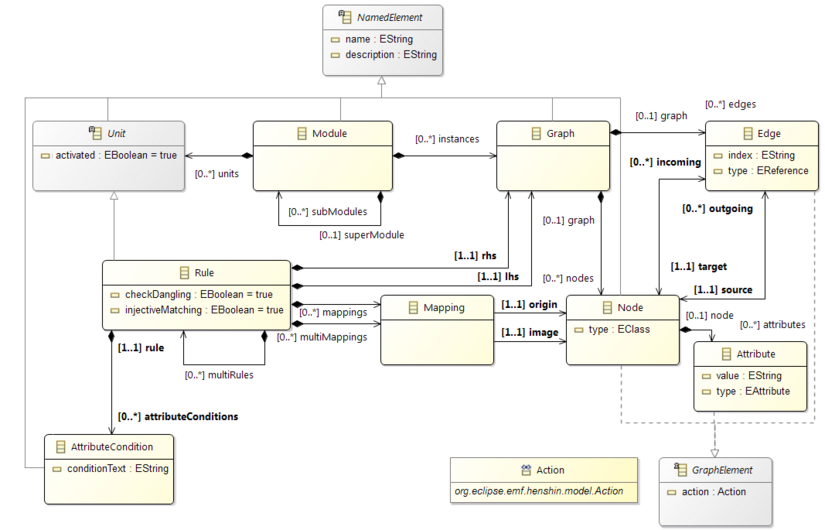
\includegraphics[width=1\textwidth]{henshin-rule-model}
    \caption{Henshin transformation rule metamodel. Image obtained from \cite{henshin-repo}}
    \label{fig:henshin-rule-model}
  \end{figure}

  \section{\acf{glsp}}
  \label{subsec:glsp}

  \ac{glsp} is a framework that provides components for the development of \acsp{gui} for web-based diagram editors.
  \cite{glsp-repo} It is organized within the Eclipse Cloud Development project. \cite{glsp-doc} With the framework, custom diagram editors for Eclipse Theia, Eclipse IDE, Visual Studio Code, or standalone web apps can be created. It uses a client-server architecture, where the client is implemented with TypeScript and for the server, GLSP provides implementations in Java and TypeScript based on nodejs, even though the server could be implemented in any programming language. As the server for this project is implemented in Java, the following discussion focuses exclusively on the Java implementation of the \ac{glsp} server. Client and server communicate over JSON-\acs{rpc} with an action protocol that is similar to the Language Server Protocol \cite{lsp-repo}. 

  The \ac{glsp} server is responsible for loading a source model and defines how to transform it into the graphical model, that should be displayed. The source model can be of any format, e.g., a database, JSON file, or an EMF model. \ac{glsp} provides dedicated modules for loading EMF models. The Java server uses Google Guice \cite{guice-repo} for \ac{di}. The \ac{glsp} server distinguishes between \ac{di} containers. There is one server \ac{di} container to configure global components that are not related to specific sessions. For every client session, there is a diagram session \ac{di} container, that holds session specific information, handlers, and states associated with a single diagram language. In Figure \ref{fig:glsp-server-di} you can see that the diagram session \ac{di} container run inside the server \ac{di} container. \ac{glsp} provides some abstract base classes that have to be implemented to create a working diagram server language, that can provide a diagram to display at the client. All concrete implementations of one diagram language have to be registered in a \code{DiagramModule}. The server can handle multiple diagram languages by providing different diagram modules. There are some classes that have to be implemented. The interface \code{SourceModelStorage} defines how to load and save the source model. There is already a default abstract implementation for \ac{emf} models, that loads the \ac{xmi} file into a \code{ResourceSet}. The interface \code{GModelFactory} is used to map the source model to the \ac{glsp} internal graphical model structure. Here also an abstract \code{EMFGModelFactory} is provided. Another important part is the \code{GModelState} interface, that defines the state of a client session and holds all information about the current state of the original source model. All services and handlers use the \code{GModelState} to obtain required information for their tasks.

   \begin{figure}[h]
    \centering
    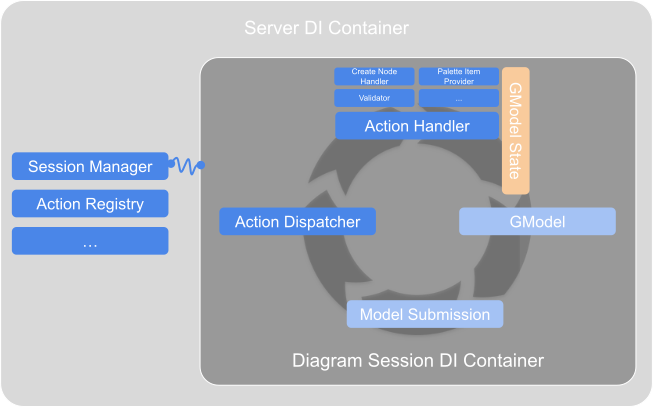
\includegraphics[width=0.7\textwidth]{glsp-server-di}
    \caption{Server DI Container vs Diagram Session DI Container. Image obtained from \cite{glsp-doc}}
    \label{fig:glsp-server-di}
  \end{figure}

  When the diagram should be displayed in the editor, the client sends a \code{RequestModelAction} with a \acs{uri} of the source model to the server. The server invokes the \code{SourceModelStorage} to load the source model and then uses the \code{GModelFactory} to translate it into the graphical model, which is then sent to the client to render it. For an edit operation, the client sends the operation request to the server, where the corresponding handler is invoked. The handler modifies the source model directly. After that, the server invokes the \code{GModelFactory} again to map the newly modified source model into a new graphical model, which is sent to the client to re-render. The two use cases share many steps. Since a new graphical model is created every time, the format of the source model is independent and can be of any format. \cite{glsp-doc}

  The \ac{glsp} client is responsible for rendering the graph and managing user interactions. The client requests all possible editing operations that can be performed on the specific model. As the client for this project is integrated into Eclipse Theia, the following discussion focuses exclusively on the Theia integration of the \ac{glsp} client. \cite{glsp-doc} \ac{glsp} provides four main \acs{ui} components to apply commands or edit the graph but also allows custom \ac{ui} extensions: 

  \begin{itemize}
    \item \textbf{ToolPalette}: The ToolPalette is an expandable \ac{ui} element located on the top left of the diagram editor. By default, it provides basic options to switch between selection, deletion, and marquee tools, validate the model, reset the viewport, and search in the listed operations below. Below it lists all nodes and edges that can be created in the diagram by default. It can be extended with custom actions by implementing and registering the \code{ToolPaletteItemProvider} interface at the server. \cite{glsp-doc,glsp-repo} 
    \item \textbf{CommandPalette}: The CommandPalette can be invoked by pressing \textit{Ctrl+Space}. It provides a search field to search for commands or actions that were registered. Commands can be registered by implementing and registering the \code{CommandPaletteActionProvider} to the server or implementing and registering the \code{CommandContribution} interface to the Theia frontend module. \cite{glsp-doc,glsp-repo} 
    \item \textbf{ContextMenu}: The ContextMenu is a popup menu that can be opened by right clicking inside the diagram editor. There, any commands or actions can be structured as needed. It can be customized by implementing and registering the \code{ContextMenuItemProvider} to the server or implementing and registering the \code{MenuContribution} interface to the Theia frontend module. \cite{glsp-doc,glsp-repo} 
    \item \textbf{EditLabelUI}: Labels of nodes and edges can be edited by double-clicking on the label. The EditLabelUI provides an input popup to edit the label text. \cite{glsp-doc,glsp-repo}
    \item \textbf{Custom \acs{ui} Components}: Custom \acs{ui} extensions have to extend \code{AbstractUIExtension} that provides a base \acs{html} element and can then be registered to the client. The base class also provides functionality to show, hide, or focus the element. These \acs{ui} extensions can also be enabled over a \code{SetUIExtensionVisibilityAction} from the server. \cite{glsp-doc,glsp-repo}
  \end{itemize}

  \ac{glsp} uses Sprotty \cite{sprotty-repo}, a web-\acs{svg}-based diagramming framework, to render the diagrams. The graphical model of \ac{glsp} called \textit{GModel} is based on the \textit{SModel} of Sprotty and works as a compatible extension. The graphical model is composed of shape elements and edges. They are organized in a tree, that starts with the \code{GModelRoot}. There are several base classes, that can be extended and also new types can be added. The \code{GEdge} represents an edge between two nodes or ports. Four classes inherit from \code{GShapeElement}, which represents an element with a certain shape, position, and size. They can also be nested inside another \code{GShapeElement}. The \code{GNode} can have \code{GLabel} or \code{GPort}, which represents a connection point for edges, as children. The \code{GCompartment} can be used as a generic container to group elements. The Java server uses \ac{emf} to handle the graphical model internally, to profit from the command-based editing capabilities of \ac{emf}. To send the graphical model to the client, it is serialized into JSON using GSON \cite{gson-repo} and then sent over JSON-\acs{rpc}. \cite{glsp-doc}

  The layout of a graph is divided into macro and micro layouting.
  The macro layouting, which arranges the nodes and edges of the model, is done by the server. The client does the micro layouting by calculating the positioning and size of elements within a container element. \cite{glsp-doc} For the macro layouting, \ac{glsp} provides a notation model, that persists the position and size of the elements in a separate notation \ac{xmi} file. The notation diagram can be added to the \code{GModelState} and then used in the \code{GModelFactory} to specify the layout. \cite{glsp-repo} \ac{glsp} also provides a \code{LayoutEngine} interface, that can be used to layout the elements of a graph that have no persisted layout yet. \cite{glsp-doc}

  \ac{glsp} also provides an interface to validate the model. With the \code{ModelValidator} interface, specific validation rules can be defined by the server. The validation returns a list of markers that can be an info, warning, or error. The markers are then displayed in the \ac{glsp} client. The markers can also be integrated into the Theia Problems View.


    \chapter{Related Work}
  \label{sec:related-work}

  \section{Scientific Literature}
  \label{subsec:related-scientific-literature}

  \section{Existing Tools and Technologies}
  \label{subsec:related-tools}

    There are many existing tools for model transformations. \citeauthor{kahani2019survey} created a survey in \citeyear{kahani2019survey} of various model transformation tools. They classified 60 different tools, including Henshin. In Figure \ref{fig:tools-environments}, you can see how many tools provide specific execution environments. 73\% of the tools provide plugins for the Eclipse \acs{ide}, and 20\% of the tools are integrated or dependent on other \acsp{ide}. 18\% have no \acs{ide} support, and only two tools are web-based. In total, 89\% of the tools have external dependencies such as an \acs{ide} or other tools. Dependencies often complicate the installation and usage of the tool. \cite{kahani2019survey}

  \begin{figure}[h]
    \centering
    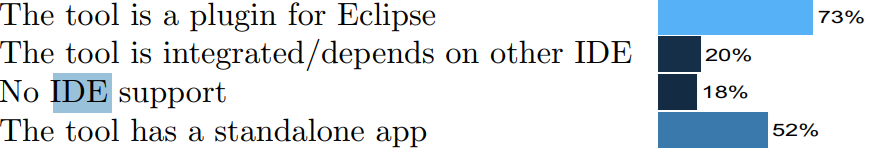
\includegraphics[width=0.6\textwidth]{model-tools.png}
    \caption{Execution environments of model transformation tools. Image obtained from \cite{kahani2019survey}}
    \label{fig:tools-environments}
  \end{figure}

  One web-based tool included in the survey is \ac{atompm} \cite{atompm}. It is a web-based modeling tool to create \ac{dsml} environments, performing model transformations and manipulating and managing models. \cite{atompm} It was created in \citeyear{atompm} and supports all model transformations that are based on T-Core \cite{tcore}, a minimal common basis that allows interoperability between different model transformation languages. \cite{tcore} Metamodels can be defined with a simplified \acs{uml} language. The graphical modeling environment offers debugging and the ability to collaborate and share modeling artifacts in the browser. \cite{atompm}


  There are also other web-based tools for \ac{mde}. WebGME \cite{webGME} is a web-based modeling tool, created in \citeyear{webGME}. It allows to collaboratively design \acp{dsml} using model versioning and broadcasting changes to all active users. It supports prototypical inheritance, where any model can be instantiated recursively, so changes are propagated down the inheritance tree. It also provides scalability, collaborative modeling and model versioning. Metamodels and compositions can be created with WebGME, but no graph transformations can be applied to a model. Even though model transformations are not possible, the editor was one of  the first solutions for web-based modeling tools. \cite{webGME} The software provides extension points to customize or extend the software, but no model transformation capabilities were added by any available extension. \cite{webgme-website} The tool is still hosted and maintained, to be used for free. \cite{webgme-website}


  WebDPF \cite{webDPF} is another web-based modeling tool, published in \citeyear{webDPF}. Compared to WebGME and \ac{atompm}, it supports model navigation and element filter capabilities, a JavaScript editor for writing predicate semantics, reusability of transformation rules, partial model completion, and a termination analysis. These features try to improve the usability of the tool. \cite{webDPF} Even though the tool had improvments upon existing tools, the originally mentioned hosted WebDPF portal is offline by now. 


  There is also a \ac{glsp}-based Ecore metamodel editor, created by the \ac{glsp} development team. It was implemented with the \ac{glsp} version 0.9 but never updated further. It allows to create and edit \ac{emf} Ecore models in a Theia web editor. Even though the project cannot be used directly, due to the use of another source model format and breaking changes in major updates of the \ac{glsp} framework, it provides various classes that can be used as a template for the Henshin Web Ecore viewer. One example is the factory code that maps the \ac{emf} Ecore model to the graphical model. \cite{glsp-ecore-repo}
  The findings show, that there are many existing model transformation tools, but only very few web-based solutions, that provide an easy entry into \ac{mde} and model transformations. Henshin web tries to fill this gap.

  \section{Comparison and Gaps}
  \label{subsec:related-comparison}

    \section{Requirements Analysis}
  \label{subsec:requirements}

  \subsection{Functional Requirements}
  \label{subsec:functional-requirements}

  The following requirements are a list of the functional and non-functional requirements (that I came up with). The client should be integrated as an Eclipse Theia client. Additional clients can be added in the future without impacting other parts of your implementation. \cite{eclipseGLSP} The backend should be implemented with Java.

  Functional requirements:

  \begin{itemize}
  
    \item \ac{emf} XMI instance files should be displayed in a graphical editor
    \item Henshin rule files should be displayed in a graphical editor
    \item \ac{emf} Ecore metafiles should be displayed in a graphical editor
    \item The instance editor should display all rules that can be applied to the instance model.
    \item Parameters of the rules should be editable when applying a rule.
    \item After applying a rule, the instance model should be updated and displayed in the instance editor as a temporal file that can be used to apply multiple rules. The initial instance model should not be changed.
    \item The instance editor should provide editing functionality for the instance model.
    \item The Henshin rule editor should provide editing functionality for the transformation rules.
    \item The Ecore editor should provide editing functionality for the Ecore metamodel.

  \end{itemize}

  Once all functional requirements are implemented, the application should fully support a basic model transformation workflow. Its functionality should be equivalent to using the Henshin plugin within the Eclipse editor. It should be possible, that additional Henshin functionalities like State Space analysis or conflict and dependency analysis can be added in the future.



  \subsection{Non-Functional Requirements}
  \label{subsec:non-functional-requirements}

  Non-functional requirements:

  \begin{itemize}
    \item The application should be web-based and accessible via a web browser.
    \item The application should be responsive and work on different screen sizes.
    \item The application should be user-friendly and intuitive to use.
    \item The application should be performant and handle large models efficiently.
\end{itemize}


  \subsection{Stakeholders and Use Cases}
  \label{subsec:stakeholders}

  \subsection{System Constraints}
  \label{subsec:system-constraints}

   \chapter{System Design and Architecture}
  \label{sec:system-design}

  In this chapter, the architecture of the system is described. The system is designed to achieve following goals. The system should be modular and easily extensible to allow future extensions towards a full model transformation platform for production use cases. The system should also be maintainable. In the folowing sections, the high-level architecture following the \ac{glsp} architecture is described. Then the design of the components, control flow and data models is described. In the end the UI design is explained.

 \section{Design Decisions}
  \label{subsec:design-decisions}

  In the section \ref{sec:background} the used frameworks and technologies were described. The selection of these framworks still leave some open design decisions. One open decision was which platform integration to use for the \ac{glsp} client. \ac{glsp} can be used as an extension for Eclipse Theia or \ac{vscode}, a plugin for the Eclipse \acs{ide} or as a standalone web application. They can also be used in combination, but to avoid overhead and complexity, only one platform integration is initially used. In table \ref{tab:glsp-platform-comparison} the different integration options are compared. Since the integration into an existing \acs{ide} fits the graph editors, the standalone editor is not an option. For that, many additional features like a file explorer have to be implemented. The integration into the Eclipse \acs{ide} is also not an option, since it is not based on web technologies and therefore not satisfying the requirements of the project. Between the Eclipse Theia and \ac{vscode} integration, Eclipse Theia is providing more flexiblity in the usage and deployment of the application. Next to the usage as an extension that can be added during runtime, Theia also provides the option to bundle your own \ac{ide} including the \ac{glsp} graph editors. That makes it deployable as a complete application, where no additional plugins are needed. This flexibility is the main reason to choose the Eclipse Theia integration as the inital main platform for Henshin Web. With that usage and deployment flexibility, different additional platform integrations are probably not needed in the future.

  \begin{table*}[h]
    \centering
    \caption{Comparison of GLSP Platform Integrations}
    \label{tab:glsp-platform-comparison}
    \resizebox{\textwidth}{!}{
        \begin{tabular}{|p{3cm}|p{3cm}|p{3cm}|p{3cm}|p{3cm}|}
            \hline
            \textbf{Criteria} & \textbf{Eclipse Theia} & \textbf{\ac{vscode}} & \textbf{Eclipse \acs{ide}} & \textbf{Standalone} \\
            \hline

            \textbf{Deployment Options} & Web-app, Desktop (Electron) & Desktop, Web-app & Desktop & Custom (Web or Desktop)\\
            \hline
            \textbf{Extendability} & Access to all Theia internal \acsp{api} & Through VS Code Extension \acsp{api} & Moderate, via Eclipse plugins (OSGi-based) & Fully customizable (with own implementations) \\
            \hline
            \textbf{Provided Environment} & Complete \acs{ide} & Complete \acs{ide} & Complete \acs{ide} & No other features included \\
            \hline
            \textbf{Result Format} & Own \acs{ide} or as a plugin & \ac{vscode} extension & Eclipse \acs{ide} plugin & javascript based web editor module \\
            \hline
            \textbf{Dependencies Needed} & browser & \ac{vscode} Desktop or browser & Eclipse \acs{ide}& browser \\
            \hline
        \end{tabular}
    }
\end{table*}



  Another decision was to select a edge routing style. \ac{glsp} provides two different routing algorithms, the Manhattan and Polylime stlyes. The Manhattan style was invented by \citeauthor{manhattan} to achieve wire length optimization in circuit design.  It only uses vertical and horizontal lines to connect nodes. \cite{manhattan}. The conncetion can be split into multiple segments, changing from a horizontal to a vertical line or the other way round to create a stair like connection between nodes. The Polyline style on the other hand uses straight lines to connect nodes. They line can also be split into multiple segments with arbitrary angles between them.
  For this use case, the main aspect is the clarity and readability of the graph. You can see the comparison of the two styles in figure \ref{fig:edge-kind-comparison}. Advantages of the Manhattan style are that can prevent edge crossings, and therefore can help reduce visual clutter. In complex diagrams with many nodes and edges, it is easier to trace the horizontal and vertical lines. On the other hand, it can overlap with other edges, which can make it hard to follow the edge. Especially named edges that overlaps partly with another edge can't be followed without clicking and highlighting it. You can see that in figure \ref{fig:edge-kind-comparison} between the \textit{Bank-Account} and the \textit{Account-Client} edge. To prevent that, the edge routing needs be stored in the notation file to be able to persist changes in the routing that remove overlapping edges. The Polyline style on the other hand is generally simpler and more compact. It can get very clutterd with many edges crossing and other nodes overlapping the diagonal lines. Metamodel, transformation rules and instances are typically not that complex, so that a simple line bewteen nodes is sufficient and additonal edge segments are not needed. Because of that, the edge placement doens't have to be stored in the notation file. The edge automatically aligns itself when a node is moved. The rotation of the edge label that it runs parallel with the line supports the simple and compact design of the Polyline style. To additionally prevent crossing lines, a option to dynammically hide the root node and its edges in \ac{xmi} graphs is introduced.

  \begin{figure}
    \centering
    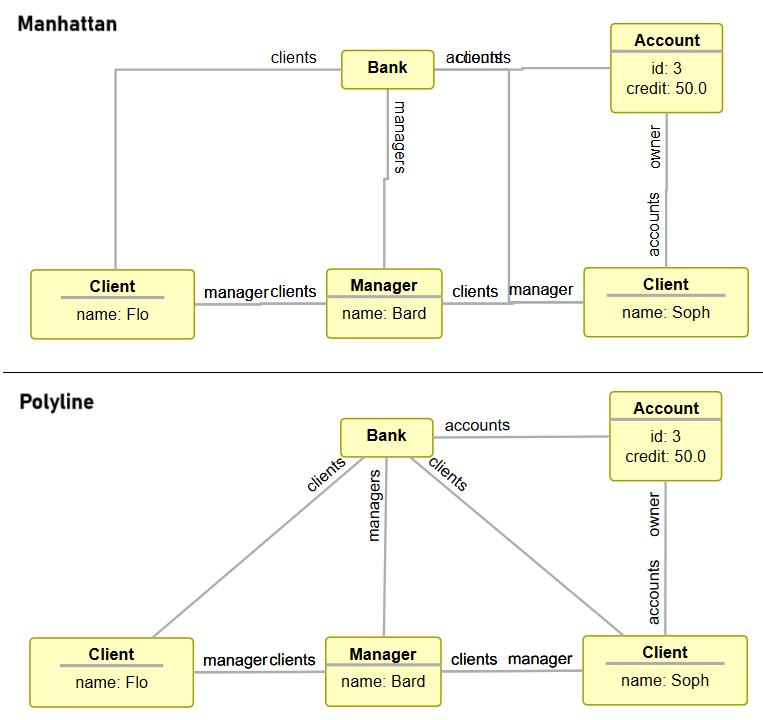
\includegraphics[width=0.7\textwidth]{edge-kind-comparison}
    \caption{Visual comparison of the two edge routing styles of \ac{glsp}}
    \label{fig:edge-kind-comparison}
  \end{figure}

    One main question in the UI design was where to put the selection of the transformation rules of a \textit{.henshin} file. There are several options to display the rule seletion. The first option is to add the list of rules to the tool palette as an additional pallete group next to the nodes and edges. Here no additional new UI element must be placed in the graph editor, but the main focus of the tool palette is to provide editing tools of the graph elements. Swapping between the rules doesn't fit into the main purpose of the tool. Another option is to create a custom UI element that is displayed in the rule graph editor. I would be easy to implement, directly integrated into the graph module and platform independent. But it would take up additional space in the graph editor view. The rule graph should be the main focus of the application and should have enough space to display the graph elements, especially for larger graphs.

    For these two options, the user also has always to switch to the rule graph editor first to select a rule. It can negatively impace toe user experience. That would not be the case if the rule selection is integrated into the Theia explorer. Since the custom explorer is used anyway to select between different instance, transformation rule or metamodel files, it is a good place to also select the transformation rules. The explorer can also be collapsed to save more space for the graphs and for very many rules it automatically supports scrolling. Extending theia internal \acs{api} makes it more effort to add aditional \ac{glsp} platform integrations, because the custom changes need to be newly implemented for the new platform, it may even not support the same extendability. Since the theia integraion provides the most options to use and deploy the application, more platform integrations are probably not needed. Aditionally, the extension of the theia explorer prevents the occupation of additional space in the \ac{glsp} editor widget to select a rule. This improvement of the user experience and intuitiveness outweights the possible additional effort for new platform integrations. The implementaiton of the custom explorer is described in section \ref{subsec:custom-ui-extensions}.


 \section{Following the \ac{glsp} Architecture}
  \label{subsec:high-level-architecture}

  The system is based on the \ac{glsp} architecture, that uses a client-server architecture. The client and server communicate via a websocket connection and JSON-RCP. The \ac{glsp} server can be implemented with Java or Node.js, but due to the constraint that Henshin is implemented in Java, the server is also implemented in Java. The client is implemented in TypeScript. \ac{glsp} provides a defined protocol for the communication between client and server, which can extended with custom commands and actions. The communication is performed using Action Messages, that can be sent from the client and the server to each other or also to itself. The client and the server have Action Handlers, that process the Action Messages and perform the corresponding actions. Each client connection starts its own server instance, therefore each server is only responsible for one client. \cite{glsp-doc} Since each client needs to be able to display three different graph editors for different file types, the server consists of three diagram modules. Each diagram module defines a different diagram language. The \code{XMIDiagramModule} is responsible for the editor of \ac{xmi} instance files, the \code{RuleDiagramModule} is responsible for the editor of Henshin rule files and the \code{EcoreDiagramModule} is responsible for the editor of Ecore metamodel files. In figure \ref{fig:architecture} you can see the high-level architecture of a server and client instance. The architecture of the three diagram modules is quite similar. Each diagram module has a \code{ModelState} which is the central statefull object within a client session \cite{glsp-doc}. The \code{ModelState} is accesed by all other services and handler and represents the current state of the actual source model. \ac{glsp} supports the integration of \ac{emf} models as the underlying source model for the diagrams by default. For that The \code{EMFSourceModelStorage} can load a \ac{emf} file as a \code{RessourceSet}, that is then attached to the \code{ModelState}. That allows an simple integration of the Henshin SDK, since it based on \ac{emf} and provides a \code{HenshinRessourceSet} can be loaded directly over the \ac{emf} integration of \ac{glsp} into the \code{ModelState}.

  The \code{ModelState} of each diagram module also contains an index and a notation model for the layout of the elements in the graphical editor. To be able to have a consistent layout of the elements, not changing after every reload or action, the position and size of each element for each model file is stored in a seperate \textit{.notation} file. The index of the \code{ModelState} is used to map the elements of the source model to the graphical model of \ac{glsp}. For each diagram module, the indexing is implemented in a different way. (see section \ref{subsec:indexing} for more details).

  Another important part of each diagram module is the \code{GModelFactory}, which is responsible for creating the graphical model that is sent to the client from the source model. Since metamodel, transformation and instance \ac{emf} model are strucutred differently, each \code{GModelFactory} of each diagram module is implementing its own mappings.

  \begin{figure}
    \centering
    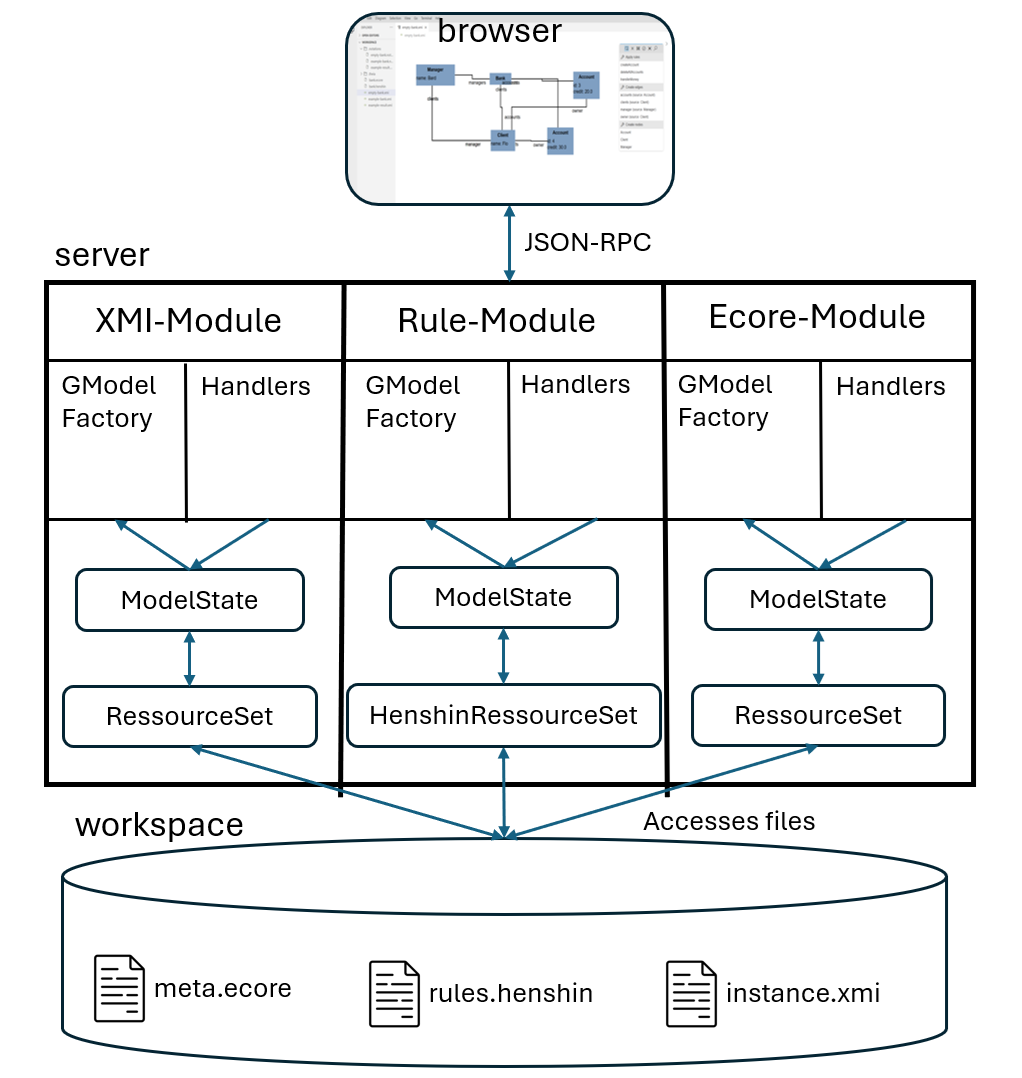
\includegraphics[width=0.6\textwidth]{architecture.png}
    \caption{High-Level Architecture of the System}
    \label{fig:architecture}
  \end{figure}

 \section{Data Models and Structures}
  \label{subsec:data-models}

  All three diagram modules have an \ac{emf} based source model. For the Ecore metamodel and the \ac{xmi} instances, The standard data model of \ac{emf} is used. As described in section \ref{subsec:emf} different implementations of \code{EObject} are used, representing all used elements like nodes, attribues or references. For the Hensin transfomations model, the data model of the Henshin \ac{sdk}, that builds upon the \ac{emf} data model, are used. No additional data structures are needed, since every created domain model is based on the \ac{emf} data model. The data model of the graphical representation is provided by \ac{glsp}. It can be extended with custom elements, but the default elements are sufficient for the current use cases. 

  The user has to select or create a workspace in the UI, where all the source models are located. Each workspace for Henshin Web has to be in a specific structure. It should contain one \textit{.ecore} metamodel and one \textit{.henshin} transformations file. Additionally, arbitrary \textit{.xmi} instance files can be added. All of these files should be stored in the root folder of the workspace. When creating a new model file or opening it for the first time, a new notation file is generated and stored in the \textit{.notation} subfolder of the workspace. These notation files are not displayed in the theia explorer.  

 \section{\ac{glsp} Client Structure}
  \label{subsec:component-design}

  The \ac{glsp} client is divided in different main modules.
  The \textit{henshin-glsp} module is responsible for platform independent code. It contains client side action handlers, custom UI extensions and custom graph elements. This module is used by the three theia specific modules, that are responsible for the integration of the \ac{glsp} client into the Eclipse Theia framework. There is one module for each diagram type. The target specific code is loacted here. One example is the customization of the Theia explorer view, that it also displays all rules of a \textit{.henshin} file and hides the notation files. These three theia extensions are then combined in the \textit{henshin-browser-app} module, that has no additional code, but only combines the three theia modules into one application. 

 \section{User Interface Design}
  \label{subsec:user-interface-design}

  The design of the user interface is based on the design principles of \ac{glsp} and Eclipse Theia. For editing the graphs, the main UI element is the tool palette on the right side of the graph editor. It lists all available nodes and edges, that can be added to the graph as well as the transformation rules that can be applied. It also contains a set of predefined \ac{glsp} actions, which are switching between selection mode, deletion mode and marquee mode, as well asreseting the viewport and search for tool palette entries. For keyboard usage, ther is also the command palette, that can be opened with the \textins{Ctrl + Space} shortcut. It opens a searchbar with a list of options below. Here all editing operations are registered listed and can be performed by searching or navigating through the list and selecting the desired operation. 
  
  The design of the custom UI elements like the parameter selection form or the display of the transformation rule information follows the design of \ac{glsp}. The design of Theia uses a flat design with minimal gradients, shadwos or 3D elements. Compared to that uses \ac{glsp} a more 3D-like design with shadows and gradients, because the UI elements need to be on top of the main graph plane. That shows that the UI elements are not part of the graph, but are additoinal elements to interact. The tool palette, comamnd pallete and context menu all use shadows and rounded eges. New custom UI elements like the parameter selection also use the same shadow and rounded corners to also show that they are not part of the graph, but elements to interact with.

  The colors of the custom UI elements follows the color theme of Theia. Important is that Theia uses the dark mode as a default theme. Graph editors typically use a light backgroung. All custom UI elements are designed to adjust to the dark mode and use the according colors as the default dark Theia elements. The final UI can be seen in appendix \ref{fig:ecore-ui}, \ref{fig:rule-ui} and \ref{fig:xmi-ui}.



  \section{Deployment and Usage}
\label{sec:deployment}

A \ac{glsp} editor can be deployed and used in production in various ways. \ac{glsp} provides platform integrations for the Eclipse Desktop IDE, Eclipse Theia, \ac{vscode}, and as a standalone web application. Each integration brings different integration possibilities, deployment, and usage options for the editor. \cite{glsp-doc} The main considerations for the deployment and usage are:
  \begin{itemize}
    \item The user should need as few dependencies as possible. Dependencies are a browser runtime, an \acs{ide} to install, or an extension to install.
    \item The app should be easy to access. Possible barriers are the creation of an account or the installation of dependencies.
    \item Using a self-hosted server or a cloud service. With a self-hosted server, the user has full access of local files to open and edit. With a cloud service, the user has to upload and download files to the server.
  \end{itemize}
  
  To use \ac{glsp} as a standalone web application, a dependency injection container with the custom \ac{glsp} client is added to a TypeScript browser application. Like that the editor of a certain file as a data source can be displayed. When the app is hosted, no other dependency than a browser runtime is needed to use the standalone diagram editor. \cite{glsp-client-repo} This option provides the most flexibility, as it can be used in any web application, but also requires the most effort to implement, when developing a complete editor. All features, like file management, window management, or other features a \acs{ide} brings, need to be implemented by the developer. \cite{glsp-client-repo} For our use case, the standalone web application is not an option, as these additional features are needed. 

  The other \ac{glsp} integrations are \acs{ide} integrations and therefore provide many features out of the box. For the Eclipse \acs{ide} integration, Eclipse has to be installed, and the \ac{glsp} plugin has to be added to the Eclipse installation. The plugin can be installed from the Eclipse Marketplace or manually by downloading the plugin jar file. \cite{eclipse-doc} The \ac{vscode} integration also provides this option. The \acs{ide} can be installed and the \ac{glsp} editor can be added as an extension. The extension can be installed from the Marketplace or manually using a \textit{.vsix} file. \cite{vscode-doc} The \ac{glsp} \ac{vscode} integration can provide a \textit{.vsix} file. \cite{glsp-repo} \ac{vscode} is the most used \acs{ide}. 73.6\% of developers use \ac{vscode} due to the survey of \citeauthor{stackoverflow2024survey} In \citeyear{stackoverflow2024survey} \cite{stackoverflow2024survey}. An advantage to Eclipse is that \ac{vscode} provides a browser version, which brings the same capabilites as the desktop \acs{ide}. \cite{vscode-doc} So this integration provides the advantage that no \acs{ide} has to be installed to be able to use Henshin Web. The user can open \ac{vscode}, add the extension, and directly open a metamodel, rule, or instance model file and start editing. 

  The Eclipse Theia \acs{ide} is not as widely popular as \ac{vscode} \cite{stackoverflow2024survey}, but its focus is not to provide a ready \acs{ide} but to provide tools to create custom \acsp{ide}. The Eclipse Theia project is part of the Eclipse Foundation and is used as a basis to create your own \acsp{ide} based on web technologies. \cite{theia-doc} They provide the Theia IDE that acts as a template editor and can be downloaded and used on all common operating systems or used in as a web editor in the browser. Due to the focus on providing a framework to build custom \acsp{ide}, Theia provides more options to use extensions and plugins to extend the functionality. You can see the options and their architectural integration into Theia in figure \ref{fig:theia-extensions}.
  \begin{itemize}
    \item \textbf{\ac{vscode} extensions} Theia provides the \ac{vscode} extension \acs{api}, so that existing \ac{vscode} extensions can be used in Theia. They only interact with the \acs{api} and therefore can be installed at runtime.
    \item \textbf{Theia plugins} are working like \ac{vscode} extensions. They interact with the Theia plugin \acs{api} and can also access the \ac{vscode} extension \acs{api}. They can access some Theia specific features, that \ac{vscode} extensions cannot access, like directly contributing to the frontend. They can also be installed at runtime, or be pre-installed at compile time.
    \item \textbf{Headless plugins} are also working like \ac{vscode} extensions. They can also be installed at runtime and can access custom extended Theia backend services.
    \item \textbf{Theia extensions} are the core architecture parts of Theia. Theia is fully built using Theia extensions in a modular way. The template Theia \acs{ide} contains Theia extensions, including the core. Custom Theia extensions can be developed and added to Theia with full access to all Theia functionality via dependency injection. They need to be installed at compile time. \cite{theia-doc}
  \end{itemize}

  The \ac{glsp} Theia integration is creating a Theia extension, that is packed into a custom Theia \acs{ide}. It is also possible to use the \ac{glsp} \ac{vscode} integration that provides a \ac{vscode} extension, that can also be added to a Theia \acs{ide} at runtime. \cite{glsp-repo} The option to use the diagram editor in the browser makes the \ac{glsp} Eclipse integration not interesting for Hensin Web. \ac{vscode} has the advantage of popularity and simplicity to use the editor without any registration or installation. Eclipse Theia has the advantage of modularity and further extensibility. Further features can be added in the future to provide a web-based environment for \ac{mde}. Theia also provides different ways to deploy a Theia \acs{ide}.   These considerations show that the Theia integration is the best option for deploying the Henshin Web editor. Theia combines the advantages of browser-based access, modularity, and extensibility.

  \begin{figure}[h]
    \centering
    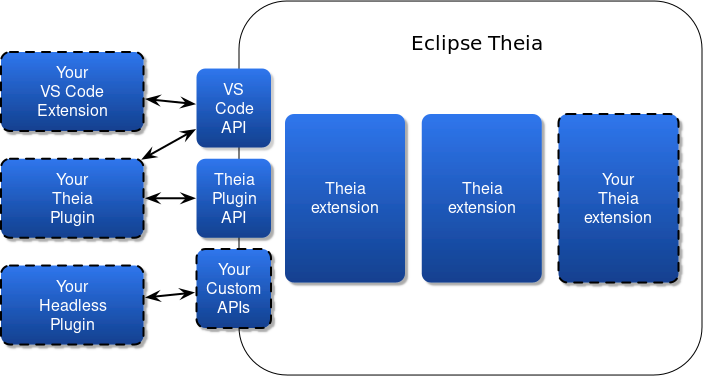
\includegraphics[width=0.7\textwidth]{theia-extension}
    \caption{Theia high level extensions and plugins architecture. Image obtained from \cite{theia-doc}}
    \label{fig:theia-extensions}
  \end{figure}

  There are different options to provide a \ac{glsp} Theia application. The Theia editor, consisting of the TypeScript client and the Java server, can be hosted in the cloud and accessed via a web browser. The Eclipse Foundation provides the Theia Cloud project \cite{theia-cloud-doc} to deploy Theia based products on Kubernetes clusters \cite{kubernetes}. Theia Cloud introduces three custom Kubernetes resource types. \textit{App Definitions} contain all necessary information about the Theia based product. \textit{Workspaces} define persistent storage solutions, where metamodel, rule, or instance model files can be stored for each user. \textit{Sessions} are acting as a runtime representaions. Theia Cloud includes components like a landing page, authentication, authorization, a cloud monitor, and a cloud operator, that deploys sessions and manages workspaces. You can see the different components and their interactions in figure \ref{fig:theia-cloud-components}. The service provides two preconfigured configurations for quickly trying out Theia Cloud on a cluster. \cite{theia-cloud-doc}

  \begin{figure}[h]
    \centering
    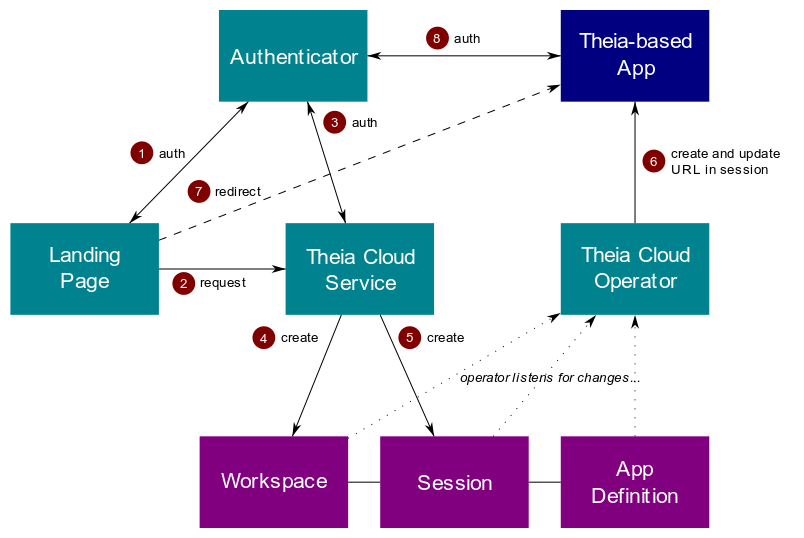
\includegraphics[width=0.7\textwidth]{theia-cloud-components.png}
    \caption{Interaction between Theia Cloud components. Image obtained from \cite{theia-cloud-doc}}
    \label{fig:theia-cloud-components}
  \end{figure}

  Because of the limited file access of the browser, the user has to upload and download all files to the server to use them. To be able to access the local file system of the user directly, the server needs to be hosted locally. For that, \ac{glsp} Theia application can be hosted in a Docker container. \cite{docker} The Docker container can contain the Java server and the TypeScript client, that are started together. The user can then access the editor via a web browser. On a machine with a Docker environment, this solution can be started locally in an easy way and has the access to the file system. The Docker container can also be used to deploy the application on a server so that it can be accessed by multiple users. The single Docker container solution doesn't provide as much scalability as using a cluster with Theia Cloud.

  The \ac{glsp} Theia application can also be used as a desktop application. Theia uses Electron \cite{electron-repo} to bundle the application into a desktop application, that can be installed via an installer. This approach also provides access to the local file system, since the electron application works like a self-hosted web application, and therefore the \ac{glsp} Java server is started locally. All in all, the \ac{glsp} Theia integration provides all different options to use the Henshin Web editor. Further clients can always be added later if needed.

  \section{Implementation}
  \label{subsec:implementation}
  This chapter describes the development process and shows the solution and implementation of specific problems, that appeared while implementing the application. The first challenge was to integrate the Henshin \acs{sdk} into the \ac{glsp} project. Another challenge was to index the elements of the different \ac{emf} models and formats. One big UI desicion was where to place the selection of transformation rules in the application.

  \subsection{Development Process}
  \label{subsec:development-process}
  The development of the Henshin Web \ac{glsp} editor was done by one person in a time span of about 6 months. Derived from the functional requirements (see section \ref{subsec:functional-requirements}) the project was split into 7 milestones. The milestones were defined as follows:
  \begin{itemize}
    \item \textbf{Milestone 1:} Setup the project and create a diagram editor that can display \textit{.xmi} files.
    \item \textbf{Milestone 2:} Create editing capabilities for \ac{xmi} instance files.
    \item \textbf{Milestone 3:} Henshin transformation rules can be displayed and applied to the instance model.
    \item \textbf{Milestone 4:} Create an additional diagram editor that can display Henshin rules.
    \item \textbf{Milestone 5:} Create an additional diagram editor that can display Ecore metamodels.
    \item \textbf{Milestone 6:} Create editing capabilities for Henshin rules.
    \item \textbf{Milestone 7:} Create editing capabilities for Ecore metamodels.
  \end{itemize}

  Each milestone was split into smaller issues. The first milestone was used to create \ac{poc} to test the integration of Henshin into a \ac{glsp} project. In this phase, the focus was to get to now how the frameworks \ac{emf}, \ac{glsp}, Henshin and Eclipse Theia work. Even though \ac{glsp} provides a well structured documentation and project templates, they didn't cover many use cases for the development of Henshin Web. Henshin also doesn't provide an documentation of their \acs{api}. Therefore for these frameworks a lot of source code reading and understanding was needed. 
  Git was used as a version control system. The development of a milestone was don in a seperate development branch. When all features of the milestone were implemented, the state of the application was additionally tested and then merged into the main branch.

  \subsection{Tooling and Environment}
  \label{subsec:tooling}
  For the development of Henshin Web, \ac{vscode} \cite{vscode} was used to develop the client and InteliJ IDEA \cite{intellij} was used to develop the Java server.
  For understanding the source code of not well documented frameworks, the use of Chatbot Agents was very helpful. I used Github Copilot in \ac{vscode} with the model Claude Sonnet 4 \cite{claude_sonnet} in agent mode. Because it has access to the source code of the dependend frameworks, it can search for specific classes or methods or explain certain concepts.
  Git was used as version control system and GitLab was used as a remote repository. It was also used for the project management, where the milestones were defined and the issues were created. A issue board was used to show the current sate and progress of the project. The GitLab package registry was also used to store the Henshin maven packages, to be able to access them from the \ac{glsp} project. These packages are then available to every contributor of the GitLab, that want to develop on the project. More about the creation on Maven packages will be shown in the next section.

  \subsection{Code Examples...}
  \label{subsec:code-examples}

  This section shows the solution and implementation of specific problems, that occured during the development process.

  \subsubsection{Integration of Henshin into a GLSP project} 
  \label{subsec:henshin-glsp}

  The Henshin source code provides both the Eclipse \ac{ide} plugin and a Java SDK for using the Henshin interpreter. The project of Henshin is structured as an Eclipse project and is available as a set of Eclipse plugins and features. \cite{henshin-repo} On the other hand, \ac{glsp} projects typically use a Maven project structure. \cite{glsp-repo} To add dependencies to a Maven project, the dependencies should ideally be available as Maven artifacts. However, Henshin doesn't provide a Maven artifact, since that is not needed for an Eclipse plugin. The Henshin version 1.8.0 is compatible with \acs{jdk} 11 and higher. \ac{glsp} version 2.3.0 has the prerequisite of \acs{jdk} 17. Therefore, the versions are compatible to run together. The Henshin code consists of 45 plugins, of which 22 are contained in the Henshin SDK, that we need as a dependency in our Henshin Web \ac{glsp} project. Each plugin can be downloaded as a \acs{jar} file. To create Maven packages from the \acsp{jar}, a PowerShell script is used. It reads all \acsp{jar} files from a folder, renames them to the correct Maven artifact name, creates a basic \code{pom.xml} file for them, deploys them to the GitLab package repository, and creates a list that needs to be included in the Maven \code{pom.xml} file of the \ac{glsp} project. A package of each plugin is created, because for the Henshin Web editor, only some parts of the Henshin SDK are needed. To use the Henshin model package, the additional dependency of the Nashorn JavaScript engine \cite{nashorn-repo} is needed. The Nashorn engine is used to execute calculation expressions of transformation rules. \cite{henshin}

  \subsubsection{GModelFactory}
  \label{subsec:gmodel-factory}

  The heart of a \ac{glsp} server diagram module is the \code{GModelFactory}. It is responsible for creating the graphical model from the source model. In listing \ref{lst:gmodel-factory} you can see the implementation of parts of the creation of the graphical nodes. The method \code{fillRootElement(GmodelRoot newRoot)} gets called when a new graphical model should be created. It fetches the source model elements from the \code{ModelState}, iterates over them, and creates \code{GNode} elements using a builder pattern. In the method \code{createNode(DynamicEObjectImpl eObject)}, it is configured how the node should look in the editor. It sets the id, adds \acs{css} classes and  configures rounded corners. It also sets the type of the node. The type can be a default type, or custom types, that have their own customized client implementation. In listing \ref{lst:gmodel-factory} you can see for example that the root node of the \ac{xmi} instance model gets a different type. The type is used to configure that only one root node can exist and that it cannot be deleted, if other child nodes exist. The method \code{applyShapeData(eObject)} adds the layout information from the notation model. In the \code{GNodeBuilder} also the builded child elements like the header or the attributes are added. This creates a tree strucutre of graphical elements, that are all atached to the \code{GModelRoot}. The \code{RuleGModelFactory} and the \code{EcoreGModelFactory} work similar to the \code{XMIGModelFactory}, but they create different node types and handle the source model elements differently.


  \subsubsection{Layouting}
  \label{subsec:layouting}

  \ac{emf} Ecore metamodel files (\textit{.ecore}), Henshin rule files (\textit{.henshin}) and \ac{emf} instance files (\textit{.xmi}), don't contain information about the position or size of elements in a graph. \cite{emf,henshin-repo} To provide a good user experience, the graphical editors need to provide a consistent macro layout for nodes and edges. Newly created nodes should not overlap with existing nodes, and the nodes should stay in the same place after reloading the editor. In general, the \ac{glsp} server is responsible for the macro layouting. \cite{glsp-doc} \ac{glsp} provides multiple options to layout the graph. The interface \code{LayoutEngine} can be used to create a custom layout algorithm, that is applied after the creation of the graphical model from the source model. \ac{glsp} provides the \code{ElkLayoutEngine} implementation, that uses the \ac{elk} to layout the graphical model. \cite{elk-engine} With \ac{elk}, different layout algorithms can be used and additionally configured. Even though \ac{elk} provides much flexibility for the layout, the layout is newly created after every change to the source model. This means that the layout is not consistent and nodes can move around after every change. To provide a consistent layout, the position of nodes need to be stored in addition to the source model. The \ac{glsp} server provides a notation model, that can be used to store the position and size of nodes and edges. \cite{glsp-repo} This brings the overhead of updating the notation model every time when the source model is updated. \ac{glsp} provides classes to make the synchronization of the notation model easier. The notation model is stored in an additional \textit{.notation} file, that is loaded together with the source model and applied to the graphical model in the \code{GModelFactory} using the \code{NotationUtil.applyShapeData(shape, builder)} method. To capture changes of position and size of nodes, the \ac{glsp} client sends the \code{ChangeRoutingPointsOperation} and \code{ChangeBoundsOperation} operations automatically when moving or resizing a node or edge. At the server, the corresponding handlers are updating the notation model using commands to provide undo and redo functionalities.

  To achieve layouting in the Henshin Web editor, notation models for the metamodel, Henshin rules, and instances are used. The \textit{.notation} file is created when the source model is loaded for the first time. Here, \ac{elk} can be used to create a fitting initial layout. For the \ac{xmi} instance models, when the graphical model gets created in the \code{GModelFactory}, the shape data from the notation model is added to the \ac{emf} elements over an \ac{emf} \code{Adapter}. Each \ac{emf} \code{EObject} has a list of adapters, that can be used to store additional information. \cite{emf} To connect the notation to an element, the \code{NotationAdapter.getOrAssignNotation()} method checks if the element already has a notation, either returning the existing notation or appending a new Adapter with the notation information.
  For the Henshin rules and the Ecore metamodels, the notation element mapping is stored in the model index that is contained in the \code{ModelState}. The reason for the different indexing approaches and their implementations will be explaine in the next section. 


  \subsubsection{Indexing EMF models}
  \label{subsec:indexing}

  Like the layout information, \ac{emf} Ecore metamodels and \ac{emf} \ac{xmi} instance models don't by default contain unique identifiers for nodes, edges, or attributes. \cite{emf,emf-repo} The graphical model of \ac{glsp} on the other hand uses identifiers for each element that is displayed. If no identifiers are specified when creating the graphical elements, \ac{glsp} generates its own internal unique identifiers. These identifiers are used in edit operations like renaming or deleting a node, where the graphical element needs to be mapped back to the source model element and only the identifier of the graphical element is sent from the client to the server. To be able to map the graphical element back to the source model element, custom identifiers need to be stored. Additionally, during the transformation of the source model into the graphical model, elements need to be accessed multiple times. For example, a source node is accessed over the \ac{emf} package when it is mapped into a \code{GNode} and then again for all its connected edges and attributes. An indexing of the elements avoid multiple lookups in the \ac{emf} source model. To be able to support any created domain meta and instance models and to prevent prerequisites for the use \ac{emf} models in Henshin Web, the \ac{glsp} server needs to create own inexes for the elements of the source model. 

  The idexing of the three different source model types is implemented in differnt ways, due to the different internal structures and stored informations. The simplest approach is used for the Henshin rule model. Henshin already creates identifiers for each node and edge of a transformation rule. These identifiers are also stored in the \textit{.henshin} file. When building the graphical model, the identifiers can be accessed over the method \code{getURIFragment(element)} of the \ac{emf} resource. When a new element is created, the index is stored in a bidirectional hash map in the \code{RuleModelIndex} that is accesible over the \code{ModelState}. This index can also be used for the notation model, where the semantic element id needs to be stored to be able to map the layout information back to the source model element. One problem of storing the Henshin identifiers is that a transformation rule is stored as a \ac{lhs} and \ac{rhs} part. Each part hs its own identifier, even though it is only one element in the graph. For that Henshin also stores mappings of the \ac{lhs} and \ac{rhs} elements in the \textit{.henshin} file. To be able to correctly map the source model elements to the graphical model elements, these mappings are also stored in the \code{RuleModelIndex}. In listing \ref{lst:rule-indexing} you can see the implementation of the methods \code{getRuleElement(id)} and \code{getRuleElementId(element)} that are used to get the element from the index or get the index of an element. You can see that before searching the index, the mapping list is checked to ensure that the \ac{lhs} element is preferably returned, if it exists. That is for example needed for setting the source and target nodes of an edge. If the edge only appears in the \ac{rhs} part and it should get deleted when applying the rule the \code{getSource()} method returns the \ac{rhs} node element, but the source node was initially created from the \ac{lhs} element. Without the mapping, the source node would not be found in the index and therefore creating an new index, that results in a invalid route in the graphical model.

  \begin{lstlisting}[language=TypeScript, caption={Parts of \code{RuleModelIndex}}, label={lst:rule-indexing}]
public void indexRuleElement(String id, GraphElement element) {
    if(ruleElementIndex.containsKey(id))
        return;
    ruleElementIndex.put(id, element);
}

public GraphElement getRuleElement(String id) {
    if (rhsToLhs.containsKey(id)) {
        String lhsId = rhsToLhs.inverseMap().get(id);
        if (ruleElementIndex.containsKey(lhsId)) {
            return ruleElementIndex.get(lhsId);
        }
    }
    return ruleElementIndex.get(id);
}

public String getRuleElementId(GraphElement element) {
    String id = element.eResource().getURIFragment(element);
    if(rhsToLhs.inverseMap().containsKey(id)){
        return rhsToLhs.inverseMap().get(id);
    }
    if(lhrToRhs.inverseMap().containsKey(id)){
        return lhrToRhs.inverseMap().get(id);
    }

    return ruleElementIndex.inverse().get(element);
}
\end{lstlisting}


  This problem doesn't appear for the Ecore metamodel indexing because no content independent indexes are stored in the \ac{emf} model. Here the indexing is used from the existing \ac{glsp} Ecore editor \cite{glsp-ecore-repo}. The \code{EcoreModelIndex} stores an index for the semantic elements, the notation elements and an additional index for inheritance edges.
  For the semantic index, random \acp{uuid} are created. They are used until the client session is closed. During this time, operations on the source model can access \ac{emf} elements by their \acp{uuid} over the stored \code{HashMap} and then apply the operation on the \ac{emf} element. The indentifiers are content-independent, which has the advantage, that the identifiers are not changing when nodes are updated. The problem with temporary identifiers on the other hand is, that they cannot be mapped to the source elements after the client session is closed. Therefore, the \acp{uuid} cannot be used in the notation model, because the same notation model needs to be loaded across client sessions. Here, the name of the \ac{emf} class is used, since it is unique for each element in the Ecore metamodel. This index has to be updated if a class is renamed.
  The inheritance index for the Ecore metamodel is used to find already created inheritance edges and retrieve their bend points. With that information, the edges can be connected at bend points to create the typical inheritance arrow structure.

  For the notation models of \ac{xmi} instance models, also content hashes are used as identifiers. Here the name of a object is not unique, because multiple objects of one class can exist. Therefore the content hash, is created from the class name and the names and values of all its attributes. A hash for the class \textit{Client} can look like this: \textit{Client:DynamicEObjectImpl-name:EString=Alice} This content hashes is generated every time the graphical model is created for the first time in a session. It needs to be updated when a attribute value is changed. Content hashes for edges would be even more complex, because they need to include the source and target node hashes combined with the edge type. This is also a reason, why the edge layout information is not stored in the notation model, since the hashes need to be changed for many edit operations to the source model. For \ac{xmi} instance elements, the additional use of adapters are used. The \code{NotationAdapter} and the \code{UUIDAdapter} store the index in the Adapter, which is then directly attaced to the \ac{emf} element. This has the advantage, especially for the \code{NotationAdapter}, that when the content hash has to be updated, the notation model can be directly fetched from the \ac{emf} element. It also contains the hashing algorithm for nodes. You can see the implementation of the \code{NotationAdapter} in listing \ref{lst:notation-adapter}. These content hashes need to be used for session independent identifiers, but using them as the only identifier would need a lot of overhead to update the hashes. Therefore, the indexing of the semantic elements works like the metamodel indexing, where \acp{uuid} are used. 
  The combination of the \acp{uuid} and content hashes allows flexibility for editing the source model, while maintaining the connection to the notation model.

  \subsubsection{Custom UI extensions}
  \label{subsec:custom-ui-extensions}

  This section demonstrates the creation of custom UI extensions by two different examples. \ac{glsp} provides a predefined interface for creating custom UI elements, that could be used in all platoform integrations. For that the abstract class \code{AbstractUIExtension} must be extended and added to the \textit{henshin-glsp} application module. One simple example is the transformation rule name with its parameters that is displayed in the top left of the rule editor. The extension needs a defined id and a parent container id. With the \code{SetUIExtensionVisibilityAction}, the UI element can be made visible from external over the id. With the method \code{initializeContents(containerElement)}, the \acs{html} elements can be created and added to the container. After the model initialization and over a public updated method, the class requests the rule name and its parameters over the \code{IActionDispatcher} and updates the UI. This update method can be called from any other class, when the \code{RuleNameUIExtension} is registered and injected over the dependency injection. One example is the explorer view, where the rule can be opened and therefore the rule name must be updated.
  
  This custom explorer is a Theia exclusive extension, accessing the Theia internal \acsp{api}. It cannot be used for other \ac{glsp} platform integrations. To use a custom theia explorer was already discussed in section \ref{subsec:design-decisions}. To implement a custom explorer, the classes \code{FileNavigatorModel}, \code{FileNavigatorTree}, and \code{FileNavigatorWidget} are extended and registered in the theia specific \textit{rules-theia} module via dependency injection. To add additional virtual elements in the explorer tree, the two new tree nodes \code{HenshinRootNode}, that contains a list of children, and \code{HenshinRuleNode}, that contains information like the rule name, are created. The method \code{resolveChildren(parent)} is overwritten in the \code{FileNavigatorTree}. Here, if it iterates over a \textit{.hensin} file node, it requests the transformation rules from the server and creates the corresponding \code{HenshinRuleNode} for each rule. It creates also an additional node that works as a \glqq{}add rule\grqq{} button. In the \code{HenshinNavigatorWidget}, the method \code{onSelectionChanged} event is subscribed. It checks if a virtual \code{HenshinRuleNode} was selected. If that is the case, it tries to find the \ac{glsp} rule wdiget and opens it. It also sends the selected rule name to the server, that is then selecting the rule in the \code{RuleGModelFactory}, where the graphical model is created. To provide a fitting look to the new tree nodes, the \code{HenshinNavigatorWidget} implements the methods \code{toNodeName(node)} and \code{toNodeIcon(node)}. Here, fitting icons are selected and the displayed names are configured.

    % \begin{lstlisting}[language=TypeScript, caption={TypeScript example}, label={lst:ts-example}]
% export class RuleNameUIExtension extends GLSPAbstractUIExtension {
%     static readonly ID = 'rule-name-ui-extension';

%     @inject(EditorContextService)
%     protected editorContext: EditorContextService;

%     @inject(TYPES.IActionDispatcher)
%     protected readonly actionDispatcher: IActionDispatcher;

%     private fullRuleString: string = '';

%     id(): string {
%         return RuleNameUIExtension.ID;
%     }
%     override containerClass(): string {
%         return RuleNameUIExtension.ID;
%     }
%     protected initializeContents(containerElement: HTMLElement): void {
%         containerElement.innerHTML = '';
%         const ruleNameElement = document.createElement('div');
%         ruleNameElement.textContent = this.fullRuleString;
%         ruleNameElement.className = 'rule-name-header';
%         containerElement.appendChild(ruleNameElement);
%     }

%     async postModelInitialization(): Promise<MaybePromise<void>> {
%         await this.setRuleName('');
%     }

%     public async setRuleName(ruleName: string): Promise<void> {
%         if (this.editorContext.diagramType === 'rule-diagram') {
%             var response = await this.actionDispatcher.request<GetParametersOfRuleResponseAction>(
%                 GetParametersOfRuleAction.create(ruleName)
%             );
%             this.fullRuleString =
%                 'Rule ' + response.ruleName + '(' + response.parameters.map(p => p.kind + ' ' + p.name + ':' + p.typeName).join(', ') + ')';

%             if (this.containerElement) {
%                 this.initializeContents(this.containerElement);
%             }
%             this.show(this.editorContext.modelRoot);
%         }
%     }

%     public async updateRuleName(ruleName: string): Promise<void> {
%         this.hide();
%         this.setRuleName(ruleName);
%     }
% }
% \end{lstlisting}


  \chapter{Testing and Evaluation}
  \label{sec:testing}

  This chapter discusses the testing strategy of the Henshin Web application. First the general strategy is described. Then the structure and results of the unit tests and end-to-end tests are seperatly presented. Finally, the limitations of the testing are discussed.

  
  \section{Testing Strategy}
  \label{subsec:testing-strategy}


The Henshin Web Model Transformation project employs a comprehensive multi-layered testing strategy to ensure reliability and correctness across both backend and frontend components. For the Java backend, unit tests were implemented using JUnit 5 framework in conjunction with Mockito for mocking dependencies. Throughout the development process, tests were incrementally added for each milestone to ensure that newly implemented functionality works as expected and does not break existing features. The test suite covers the core functionality of the backend, including model operations, rule transformations, and handler implementations. Mocking was extensively used to simulate the behavior of complex components such as the ModelState, EditingDomain, and various EMF resources, allowing for isolated testing of individual components without dependencies on external systems.

To test the user interface and end-to-end functionality, automated UI tests were created using Playwright framework. This choice was made after evaluating several alternatives including Cypress and Selenium, with Playwright being selected for its robust support of Theia applications through the specialized @theia/playwright testing library. The testing strategy ensures both individual component reliability through unit testing and complete system functionality through comprehensive end-to-end testing scenarios.

  \section{Unit Tests}
  \label{subsec:test-results}


The backend unit testing suite comprises 46 individual test files covering all critical components of the GLSP server implementation. The tests are organized into several key areas: base functionality tests verify core constants and utility classes like HenshinTypesTest, model layer tests ensure proper functioning of components such as RuleModelIndex and various factory classes, handler tests validate the correct behavior of operation handlers for actions like rule updates and model modifications, and XMI processing tests confirm proper handling of model transformations and rule applications.

The unit tests employ sophisticated mocking strategies using Mockito to isolate components under test. For instance, the RuleModelIndexTest uses mock EObject instances and EMFSemanticIdConverter to test model indexing functionality without requiring actual EMF resources. Similarly, handler tests like UpdateRuleOperationHandlerTest mock complex dependencies such as RuleModelState and ActionDispatcher while using real Henshin test resources for integration-style testing. A dedicated TestHelper class provides standardized test resource management, loading consistent test models including bank.ecore, bank-instance.xmi, and bank.henshin files across all test cases.

The tests maintain high coverage of critical paths including error handling, edge cases, and boundary conditions. For example, tests verify proper exception handling when resources cannot be loaded, validate parameter mapping functionality with empty and populated data sets, and ensure correct behavior when operating on invalid or missing model elements. The use of JUnit 5's advanced features such as parameterized tests and conditional test execution allows for comprehensive validation across different scenarios and configurations.

  \section{E2E Tests}
  \label{subsec:performance-evaluation}

For end-to-end testing, different frameworks were initially considered including Cypress, Playwright, Selenium, and several others. After careful evaluation considering factors such as Theia application support, test reliability, debugging capabilities, and maintenance overhead, Playwright was selected as the optimal choice. The decision was further reinforced by the availability of the specialized @theia/playwright library, which provides native support for testing Theia-based applications with built-in helpers for common operations and better handling of Theia's asynchronous loading behavior.

The E2E test suite encompasses three main test files covering distinct aspects of the application: app.spec.ts validates basic application loading and ensures the main content panel is visible after startup, explorer.spec.ts tests the file explorer functionality including navigation, file selection, and workspace operations, and xmi.spec.ts provides comprehensive testing of the GLSP diagram editor including XMI file opening, diagram element rendering, user interactions, and context menu operations. The tests are configured with extended timeouts to accommodate the complex loading sequences of GLSP editors and include comprehensive error handling with screenshot capture and video recording for failed test scenarios.

The E2E tests simulate realistic user workflows such as opening the bank example workspace, navigating to XMI files, launching the GLSP diagram editor, interacting with diagram elements, and validating that model transformations are properly reflected in the visual representation. The test configuration supports multiple browsers including Chromium and Firefox, ensuring cross-browser compatibility. Advanced features such as trace collection on retry, automatic screenshot capture on failure, and video recording provide comprehensive debugging information when tests fail, significantly reducing the time required to diagnose and fix issues.

  \section{Limitations}
  \label{subsec:user-feedback}

  While the testing strategy provides comprehensive coverage, several limitations were identified during implementation and execution. The E2E tests are inherently dependent on the complete application stack being operational, including the Theia frontend, GLSP server, and all associated services, making them more fragile and slower to execute than unit tests. The complex asynchronous nature of GLSP editors occasionally leads to timing-related test failures, particularly in CI environments with limited resources, requiring careful timeout management and retry logic.

The unit test mocking strategy, while effective for isolation, sometimes masks integration issues that only surface when components interact with real EMF resources and editing domains. Some complex model transformation scenarios are difficult to test in isolation and require comprehensive integration tests that bridge the gap between unit and E2E testing. Additionally, the current test suite has limited coverage of performance scenarios and stress testing, focusing primarily on functional correctness rather than system behavior under load.

The testing infrastructure requires significant setup and maintenance overhead, particularly for the E2E tests which depend on specific versions of browsers, the Theia framework, and associated testing libraries. Browser compatibility testing is limited to Chromium and Firefox, potentially missing issues specific to other browser engines. Finally, while the test suite provides good coverage of happy path scenarios and common error cases, coverage of edge cases involving malformed models or unusual user interaction patterns could be expanded to further improve system robustness.


  \chapter{Discussion}
  \label{sec:discussion}

  \section{Interpretation of Results}
  \label{subsec:interpretation-results}

  \section{Challenges and Limitations}
  \label{subsec:challenges-limitations}

  \section{Conclusion and Future Work}
  \label{sec:conclusion}

  \section{Summary of Contributions}
  \label{subsec:summary-contributions}

  \section{Suggestions for Future Development}
  \label{subsec:suggestions-future-development}

  Edapt

  \newpage
\section{Acronyms}
\label{sec:acronyms}
\begin{acronym}[AToMPM]
    \acro{glsp}[GLSP]{Graphical Language Server Platform}
    \acro{emf}[EMF]{Eclipse Modeling Framework}
    \acro{mde}[MDE]{Model-Driven Engineering}
    \acro{gui}[GUI]{Graphical User Interface}
    \acro{ide}[IDE]{Integrated Development Environment}
    \acro{sdv}[SDV]{Software-Defined Vehicle}
    \acro{jdt}[JDT]{Java Development Tools}
    \acro{pde}[PDE]{Plug-in Development Environment}
    \acro{sdk}[SDK]{Software Development Kit}
    \acro{api}[API]{Application Programming Interface}
    \acro{uml}[UML]{Unified Modeling Language}
    \acro{xmi}[XMI]{XML Metadata Interchange}
    \acro{xml}[XML]{Extensible Markup Language}
    \acro{lhs}[LHS]{Left-Hand Side}
    \acro{rhs}[RHS]{Right-Hand Side}
    \acro{nac}[NAC]{Negative Application Condition}
    \acro{pac}[PAC]{Positive Application Condition}
    \acro{rpc}[RPC]{Remote Procedure Call}
    \acro{di}[DI]{Dependency Injection}
    \acro{html}[HTML]{Hypertext Markup Language}
    \acro{svg}[SVG]{Scalable Vector Graphics}
    \acro{uri}[URI]{Uniform Resource Identifier}
    \acro{jdk}[JDK]{Java Development Kit}
    \acro{jar}[JAR]{Java Archive}
    \acro{elk}[ELK]{Eclipse Layout Kernel}
    \acro{poc}[POC]{Proof of Concept}
    \acro{uuid}[UUID]{Universally Unique Identifier}
    \acro{atompm}[AToMPM]{A Tool for Multi-Paradigm Modeling}
    \acro{dsml}[DSML]{Domain Specific Modeling Language}
    \acro{vscode}[VS Code]{Visual Studio Code}
    \acro{css}[CSS]{Cascading Style Sheets}
  \end{acronym}

  \section{Appendix}
  \label{sec:appendix}

  \begin{figure}[H]
    \centering
    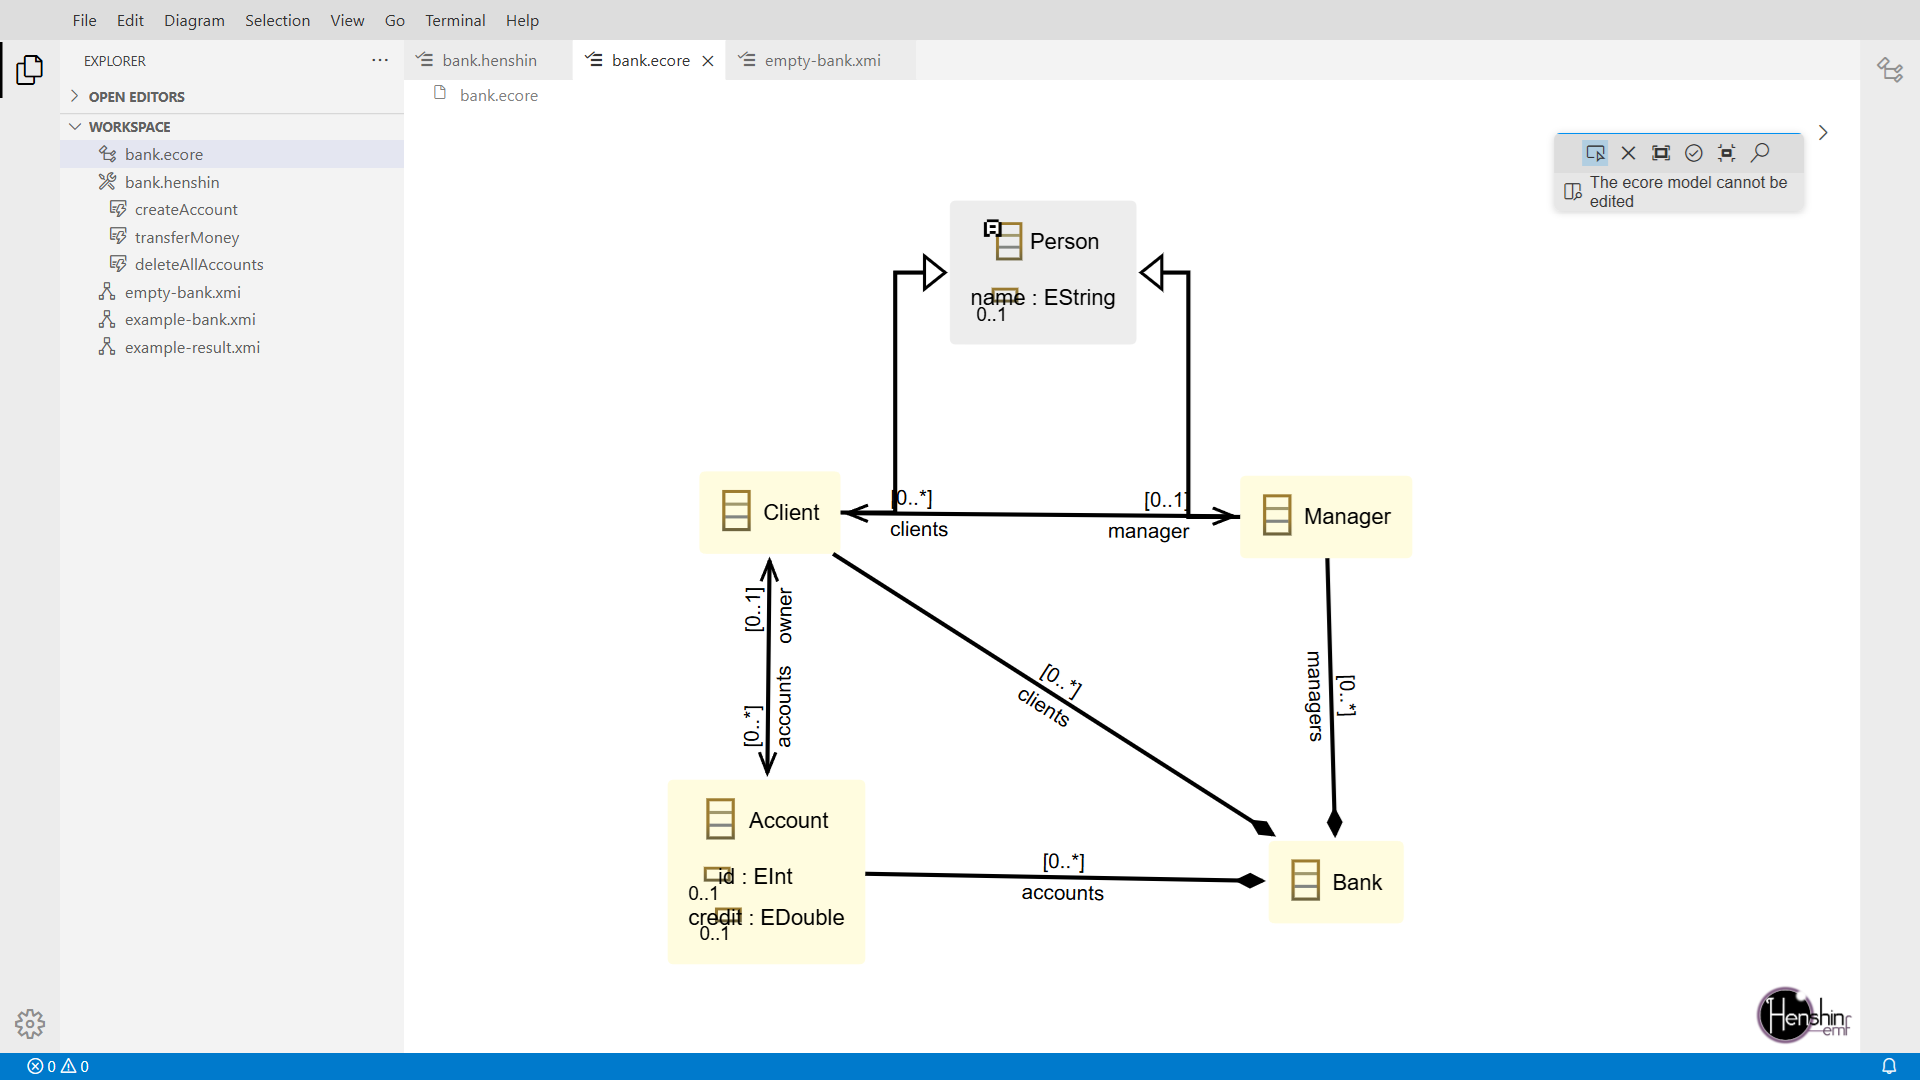
\includegraphics[width=1\textwidth]{ecore-ui}
    \caption{Henshin Web Ecore graph editor}
    \label{fig:ecore-ui}
  \end{figure}

  \begin{figure}[H]
    \centering
    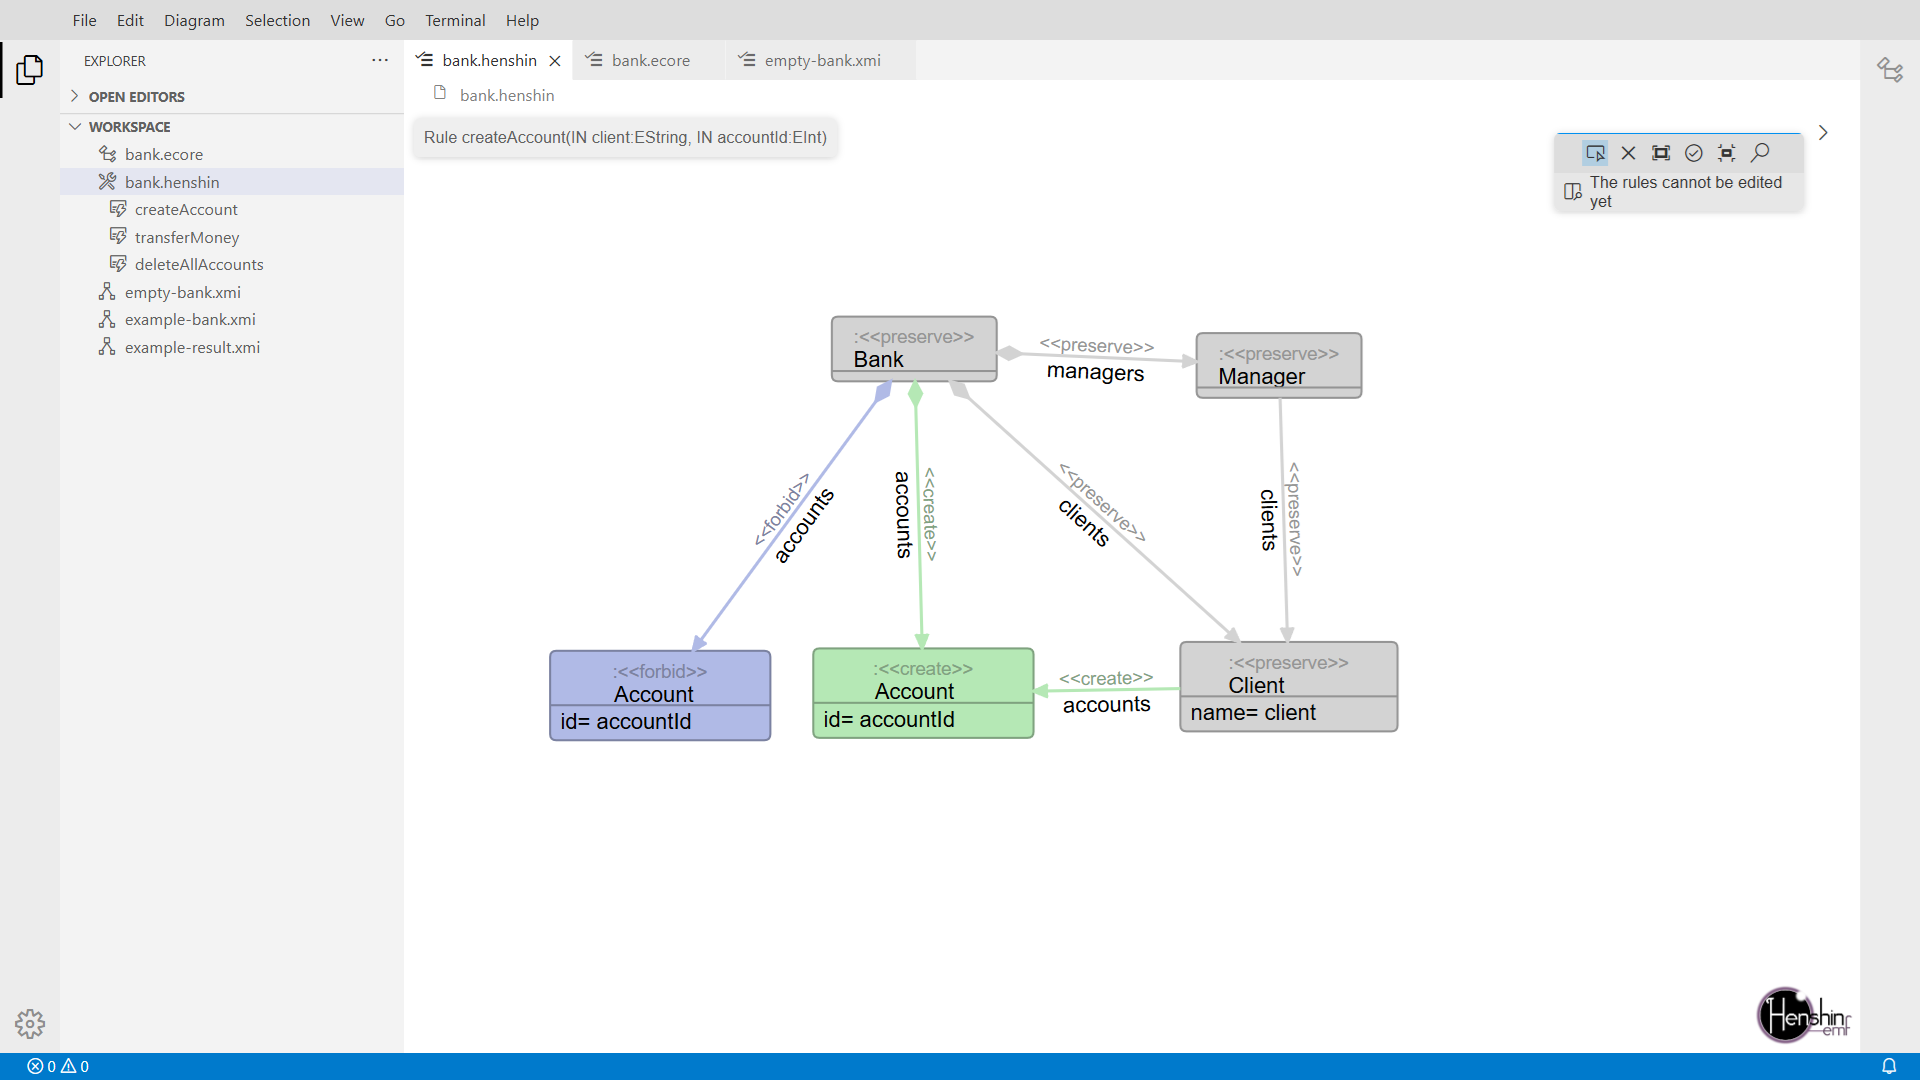
\includegraphics[width=1\textwidth]{rule-ui}
    \caption{Henshin Web Rules graph editor}
    \label{fig:rule-ui}
  \end{figure}

  \begin{figure}[H]
    \centering
    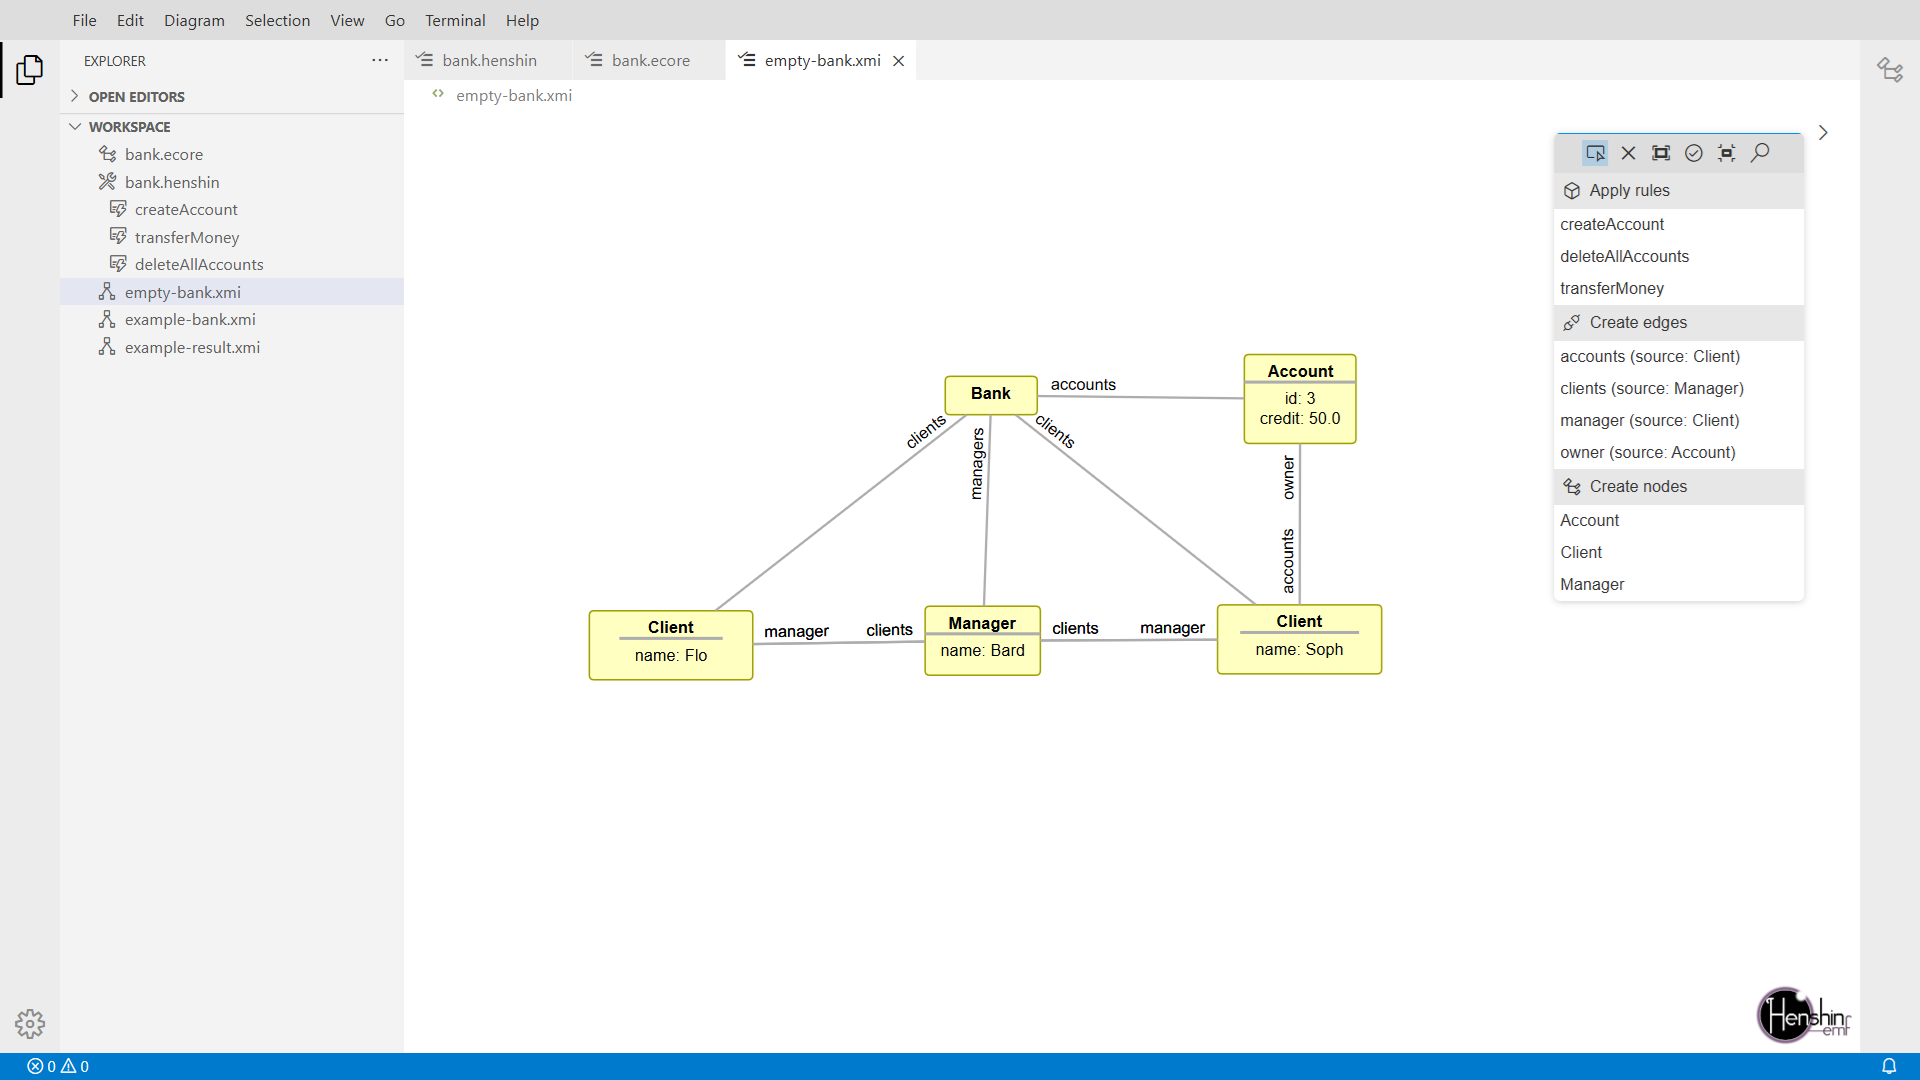
\includegraphics[width=1\textwidth]{xmi-ui}
    \caption{Henshin Web Instance graph editor}
    \label{fig:xmi-ui}
  \end{figure}



  
  \printbibliography

\end{document}
